%================================================================%
%======  Modelo de Monografia ( UFOP - DECOM) ===================%
% Proposta de texto em conformidade com normas da ABNT ----------%
% implementadas pelo projeto abntex2, que pode ser acessado pela %
% página  http://abntex2.googlecode.com/  -----------------------%
%================================================================%
\documentclass[12pt, % tamanho da fonte
   %openright,	     % capítulos começam em página ímpar
	oneside,		  % twoside para impressão em frente e verso.  
	a4paper,			% tamanho do papel. 
	english,			% Idioma adicional para hifenização
    brazil,				% Idioma principal 
    sumario=tradicional % Comente para o sumário ser conforme a opção padrão recomendada pela ABNT NBR 6027:2012.
	]{abntex2}

%------------------------------------------------------------
%------------    Estrutura do texto   -----------------------      

% Pacotes Básicos:
\usepackage[T1]{fontenc}		% Seleção de códigos de fonte.
\usepackage[utf8]{inputenc}		% Codificação do documento (conversão automática dos acentos)
\usepackage{lastpage}		    % Usado pela Ficha catalográfica
\usepackage{indentfirst}		
\usepackage{color}				% Controle das cores
\usepackage{graphicx}			% Inclusão de gráficos
\usepackage{tabularx}
\usepackage{microtype} 		  	% Melhorias da justificação
\usepackage{pdfpages}           %inserir páginas em PDF
% Pacotes Extras:
\usepackage{amsmath,amsthm}     % Símbolos Matemáticos
\usepackage[portuguese, ruled, linesnumbered,commentsnumbered, algo2e, vlined, lined, boxed, algochapter]{algorithm2e} % Algoritmos 
\usepackage{hyperref}      % Criação de links.

% Escolha da formatação das referências Bibliográficas: 
\usepackage[alf,abnt-etal-list=0,abnt-etal-cite=3]{abntex2cite}	% Citações padrão ABNT  (AUTOR, ANO)
\usepackage{etoolbox}
%\usepackage[num]{abntex2cite}  % Citações numéricas (1)
%\citebrackets[] % Usar este comando para a citação numérica aparecer com [].

% Numeração das Figuras e Tabelas
\counterwithin{figure}{chapter}
\counterwithin{table}{chapter}

% Defininção de Cores:
\definecolor{blue}{RGB}{25,25,112}
\makeatletter % informações do PDF
\hypersetup{
    %pagebackref= false,
	pdftitle={\@title}, 
	pdfauthor={\@author},
    %pdfsubject={\imprimirpreambulo},
	pdfcreator={LaTeX with abnTeX2},
	pdfkeywords={abnt}{latex}{abntex}{abntex2}{trabalho acadêmico}, 
	colorlinks=true,    % false: boxed links; true: colored links
    linkcolor=blue,     % color of internal links
    citecolor=blue,     % color of links to bibliography
    filecolor=magenta, 	% color of file links
	urlcolor=blue,
	bookmarksdepth=4
}
\makeatother

% -------------------------------------------- 
% Espaçamentos entre linhas e parágrafos 
\setlength{\parindent}{1.3cm} % O tamanho do parágrafo

% Controle do espaçamento entre um parágrafo e outro:
\setlength{\parskip}{0.2cm}  % tente também \onelineskip

% Definição de ambientes matemáticos em português 
\newtheorem{teorema}{Teorema}[chapter]
\newtheorem{axioma}{Axioma}[chapter]
\newtheorem{corolario}{Corolário}[chapter]
\newtheorem{lema}{Lema}[chapter]
\newtheorem{proposicao}{Proposição}[chapter]
\newtheorem{definicao}{Definição}[chapter]
\newtheorem{exemplo}{Exemplo}[chapter]
\newtheorem{observacao}{Observação}[chapter]

% Novos Comandos
\usepackage{tgtermes}
\renewcommand{\ABNTEXchapterfont}{\rmfamily\bfseries}

% Variáveis adicionais
\providecommand{\imprimirautorcite}{}
\newcommand{\autorcite}[1]{\renewcommand{\imprimirautorcite}{#1}} 
\providecommand{\imprimirsubtitulo}{}
\newcommand{\subtitulo}[1]{\renewcommand{\imprimirsubtitulo}{#1}} 
\providecommand{\imprimirsigla}{}
\newcommand{\sigla}[1]{\renewcommand{\imprimirsigla}{#1}}
\providecommand{\imprimiruf}{}
\newcommand{\uf}[1]{\renewcommand{\imprimiruf}{#1}}
\providecommand{\imprimircurso}{}
\newcommand{\curso}[1]{\renewcommand{\imprimircurso}{#1}}
\providecommand{\imprimirinstituto}{}
\newcommand{\instituto}[1]{\renewcommand{\imprimirinstituto}{#1}}
\providecommand{\imprimirdepartamento}{}
\newcommand{\departamento}[1]{\renewcommand{\imprimirdepartamento}{#1}}
\providecommand{\imprimirano}{}
\newcommand{\ano}[1]{\renewcommand{\imprimirano}{#1}}
\providecommand{\imprimirgrau}{}
\newcommand{\grau}[1]{\renewcommand{\imprimirgrau}{#1}}
\providecommand{\imprimirexaminadorum}{}
\newcommand{\examinadorum}[1]{
    \renewcommand{\imprimirexaminadorum}{#1}}
\providecommand{\imprimirexaminadordois}{}
\newcommand{\examinadordois}[1]{
    \renewcommand{\imprimirexaminadordois}{#1}}
\providecommand{\imprimirexaminadortres}{}
\newcommand{\examinadortres}[1]{
    \renewcommand{\imprimirexaminadortres}{#1}}
\providecommand{\imprimirexaminadorquatro}{}
\newcommand{\examinadorquatro}[1]{
    \renewcommand{\imprimirexaminadorquatro}{#1}}
\providecommand{\imprimirttorientador}{}
\newcommand{\ttorientador}[1]{
    \renewcommand{\imprimirttorientador}{#1}} 
\providecommand{\imprimirttcoorientador}{}
\newcommand{\ttcoorientador}[1]{
    \renewcommand{\imprimirttcoorientador}{#1}}
\providecommand{\imprimirttexaminadorum}{}
\newcommand{\ttexaminadorum}[1]{
    \renewcommand{\imprimirttexaminadorum}{#1}}
\providecommand{\imprimirttexaminadordois}{}
\newcommand{\ttexaminadordois}[1]{\renewcommand{
        \imprimirttexaminadordois}{#1}}
\providecommand{\imprimirttexaminadortres}{}
\newcommand{\ttexaminadortres}[1]{
    \renewcommand{\imprimirttexaminadortres}{#1}}
\providecommand{\imprimirttexaminadorquatro}{}
\newcommand{\ttexaminadorquatro}[1]{
    \renewcommand{\imprimirttexaminadorquatro}{#1}}
		
%----------------------------------------------------
\renewcommand{\imprimircapa}{ % Capa 
\begin{capa}
        \begin{center}
                \begin{DoubleSpace}
                \MakeUppercase{\imprimirinstituicao } \\
                 \MakeUppercase{\imprimirinstituto } \\
                \MakeUppercase{\imprimirdepartamento} \\
                \end{DoubleSpace}
                \vspace{5cm}
				\MakeUppercase{\imprimirautor}  \\
                \imprimirorientadorRotulo ~\imprimirorientador \\
                \imprimircoorientadorRotulo ~\imprimircoorientador \\
                        				
				\vspace{5cm}
             \textbf{{\large\MakeUppercase{\imprimirtitulo}}} \\
			 \textbf{{\large \MakeUppercase{\imprimirsubtitulo}}} \\
				\vfill
        {\large{\imprimirlocal, ~\imprimiruf \\ \imprimirano  }}
        \end{center}
\end{capa}   
} % Capa



%----------------------------------------------------
\renewcommand{\imprimirfolhaderosto}{% folha de rosto
       \begin{center}
                \MakeUppercase{\imprimirinstituicao } \\
                 \MakeUppercase{\imprimirinstituto } \\
                \MakeUppercase{\imprimirdepartamento} \\
                
                \vspace{4cm}
				\MakeUppercase{\imprimirautor}  \\
				\vspace{2cm}
			    \begin{DoubleSpace}
                \MakeUppercase{\textbf{\imprimirtitulo} } \\
                \MakeUppercase{\textbf{\imprimirsubtitulo}} \\
                \end{DoubleSpace} 
      \end{center}
    \vfill 
    \begin{flushright} 
    \parbox{0.6\linewidth}{
    Proposta de TCC submetida para a aprovação na matéria de Introdução ao TCC, requisito parcial para obtenção do grau de Bacharel em Ciências da Computação pela Universidade Federal de Santa Catarina.\\ \\
% 		\imprimirtipotrabalho~ apresentada ao Curso de \imprimircurso~ da \imprimirinstituicao~ como parte dos
% 		requisitos necessários para a obtenção do grau de \imprimirgrau. \\ \\
		\textbf{\imprimirorientadorRotulo}~\imprimirorientador \\
		
		\textbf{\imprimircoorientadorRotulo}~\imprimircoorientador}
   \end{flushright} 
		\vfill
   \begin{center}
   {\large{\imprimirlocal, ~ \imprimiruf \\
   \imprimirano} }
   \end{center} }  % folha de rosto

%----------------------------------------------------


 % Estrutura do documento e pacotes usados. Outros pacotes (packages) devem ser  adicionados ao arquivo structure.tex. 

% -- Informações para Capa e Folha de Rosto: ---------------
\titulo{Revisão de Percepções} 
\subtitulo{}
\autor{Gustavo Emanuel Kundlatsch} \autorcite{Aluno, Gustavo Emanuel Kundlatsch}
\local{Florianópolis} \uf{Santa Catarina}
\data{21 de agosto de 2020} \ano{2020}
\orientador{Me. Thiago Ângelo Gelaim}  % Nome do orientador. Caso seja uma orientadora use o comando ∖orientador[Orientadora:]{Nome}
\ttorientador{Universidade Federal de Santa Catarina} % Instituição do orientador
\coorientador{Prof. Dr. Elder Rizzon Santos}   % Nome do coorientador
\ttcoorientador{Universidade Federal de Santa Catarina} % Instituição do Coorientador
\instituicao{Universidade Federal de Santa Catarina} \sigla{UFSC}
\instituto{Centro Tecnológico}
\departamento{Departamento de Informática e Estatística}
\curso{Ciência da Computação}	
\tipotrabalho{Monografia} % Monografia (Monografia II)
\grau{Bacharel em Ciência da Computação}

%------Nomes dos membros da banca.  
\examinadorum{Prof. Dr. Membro da Banca 1}
\ttexaminadorum{Universidade Federal de ... - UFXX}
\examinadordois{Prof. Dr. Membro da Banca  2}
\ttexaminadordois{Universidade Federal de ... - UFXX}
%\examinadortres{Prof. Dr. Membro da Banca  3} 
\ttexaminadortres{Universidade Federal de ... - UFXX}
%\examinadorquatro{Prof. Dr. Membro da Banca  4}
\ttexaminadorquatro{Universidade Federal de ... - UFXX}



% MEUS PACOTES

\usepackage{booktabs}
\usepackage{graphicx}
\usepackage{enumitem}
\usepackage{csquotes}
\usepackage[linesnumbered]{algorithm2e}
\usepackage{amsthm}
\usepackage{amssymb}
\usepackage{verbatim}
\usepackage{amsmath}
\usepackage{caption}
\usepackage{algorithm}
\usepackage{tocbibind}

 \usepackage[table,xcdraw]{xcolor}
 

\newcolumntype{Y}{>{\centering\arraybackslash}X}

\theoremstyle{definition}
\newtheorem{definition}{Definição}
\newtheorem{example}{Exemplo}[section]

% SIGON
\usepackage{listings}
\renewcommand{\lstlistingname}{Código}
\usepackage{xcolor}
\lstset{%
    language=Python,
    basicstyle=\small\ttfamily,%
    numbers=left, numberstyle=\tiny, stepnumber=1, numbersep=5pt,%
    aboveskip=3mm,
    belowskip=3mm,
    showstringspaces=false,
    columns=flexible,
        morekeywords={plan, action, sensor, actuator, sense, member},
    basicstyle={\small},
    numberstyle=\tiny\color{gray},
    keywordstyle={[2]\color{blue}},
    keywordstyle={[3]\color{red}},
    keywordstyle={[4]\color{black}},
    otherkeywords={String,async,await,Task,var},
    keywords=[2]{communication, beliefs, desires, intentions, planner},
    keywords=[3]{:},
    keywords=[4]{sensor, actuator},
    commentstyle=\color{ForestGreen},
    stringstyle=\color{red},
    captionpos=b, 
    breaklines=true,
    breakatwhitespace=true,
    tabsize=3
}%

% ------------------------------------------------------
\makeindex   

\begin{document} % Início do documento

\frenchspacing  % Retira espaço obsoleto entre as frases.

% ----------------------------------------------------------
% -- Elementos Pré-Textuais: -------------------------------
\pagenumbering{roman}

\imprimircapa  % Capa
\imprimirfolhaderosto % Folha de rosto
\begin{table}[H]
\centering
\begin{tabular}{ll}
\multicolumn{2}{c}{\cellcolor[HTML]{C0C0C0}\textbf{FOLHA DE APROVAÇÃO DE PROPOSTA DE TCC}}                \\ \hline
\multicolumn{1}{|l|}{\textbf{Acadêmico}}            & \multicolumn{1}{l|}{Gustavo Emanuel Kundlatsch}              \\ \hline
\multicolumn{1}{|l|}{\textbf{Título do trabalho}} &
  \multicolumn{1}{l|}{\begin{tabular}[c]{@{}l@{}}Revisão de Percepções\end{tabular}} \\ \hline
\multicolumn{1}{|l|}{\textbf{Curso}}                & \multicolumn{1}{l|}{Ciência da Computação/INE/UFSC} \\ \hline
\multicolumn{1}{|l|}{\textbf{Área de Concentração}} & \multicolumn{1}{l|}{Inteligência Artificial}                    \\ \hline
\end{tabular}%
\end{table}
\noindent
\textbf{Instruções para preenchimento pelo \underline{ORIENTADOR DO TRABALHO}:}

\noindent - Para  cada  critério avaliado,  assinale  um  X  na  coluna  SIM  apenas  se  considerado  aprovado.

\noindent Caso contrário, indique as alterações necessárias na coluna Observação.
\begin{table}[H]
\resizebox{\textwidth}{!}{%
\begin{tabular}{|l|
>{\columncolor[HTML]{C0C0C0}}l |
>{\columncolor[HTML]{C0C0C0}}l |
>{\columncolor[HTML]{C0C0C0}}l |
>{\columncolor[HTML]{C0C0C0}}l |l|}
\hline
\multicolumn{1}{|c|}{\cellcolor[HTML]{C0C0C0}} &
  \multicolumn{4}{c|}{\cellcolor[HTML]{C0C0C0}\textbf{Aprovado}} &
  \cellcolor[HTML]{C0C0C0} \\ \cline{2-5}
\multicolumn{1}{|c|}{\multirow{\cellcolor[HTML]{C0C0C0}\textbf{Critérios}}} &
  \multicolumn{1}{c|}{\cellcolor[HTML]{C0C0C0}\textbf{Sim}} &
  \multicolumn{1}{c|}{\cellcolor[HTML]{C0C0C0}\textbf{Parcial}} &
  \multicolumn{1}{c|}{\cellcolor[HTML]{C0C0C0}\textbf{Não}} &
  \multicolumn{1}{c|}{\cellcolor[HTML]{C0C0C0}\textbf{\begin{tabular}[c]{@{}c@{}}Não \\ se aplica\end{tabular}}} &
  \multirow{\cellcolor[HTML]{C0C0C0}\textbf{Observação}} \\ \hline
\begin{tabular}[c]{@{}l@{}}1. O trabalho é adequado para um TCC no \\ CCO/SIN (relevância / abrangência)?\end{tabular} &
   &
   &
   &
   &
   \\ \hline
2. O titulo do trabalho é adequado? &
   &
   &
   &
   &
   \\ \hline
3. O tema de pesquisa está claramente descrito? &
   &
   &
   &
   &
   \\ \hline
\begin{tabular}[c]{@{}l@{}}4. O problema/hipóteses de pesquisa do\\ trabalho está claramente identificado?\end{tabular} &
   &
   &
   &
   &
   \\ \hline
5. A relevância da pesquisa é justificada? &
   &
   &
   &
   &
   \\ \hline
\begin{tabular}[c]{@{}l@{}}6. Os objetivos descrevem completa e\\ claramente o que se pretende alcançar neste trabalho?\end{tabular} &
   &
   &
   &
   &
   \\ \hline
\begin{tabular}[c]{@{}l@{}}7. É definido o método a ser adotado no\\ trabalho? O método condiz com os objetivos e \\ é adequado para um TCC?\end{tabular} &
   &
   &
   &
   &
   \\ \hline
\begin{tabular}[c]{@{}l@{}}8. Foi definido um cronograma coerente com \\ o método definido (indicando todas as\\ atividades) e com as datas das entregas\\ (p.ex. Projeto I, II, Defesa)?\end{tabular} &
   &
   &
   &
   &
   \\ \hline
\begin{tabular}[c]{@{}l@{}}9. Foram identificados custos relativos \\ à execução deste trabalho (se houver)?\\ Haverá financiamento para estes custos?\end{tabular} &
   &
   &
   &
   &
   \\ \hline
\begin{tabular}[c]{@{}l@{}}10. Foram identificados todos os envolvidos\\ neste trabalho?\end{tabular} &
   &
   &
   &
   &
   \\ \hline
\begin{tabular}[c]{@{}l@{}}11. As formas de comunicação foram\\ definidas (ex: horários para orientação)?\end{tabular} &
   &
   &
   &
   &
   \\ \hline
\begin{tabular}[c]{@{}l@{}}12. Riscos potenciais que podem causar\\ desvios do plano foram identificados?\end{tabular} &
   &
   &
   &
   &
   \\ \hline
\begin{tabular}[c]{@{}l@{}}13.  Caso o TCC envolva a produção de um \\ software ou outro tipo de produto e seja \\ desenvolvido também como uma atividade \\ realizada numa empresa ou laboratório, \\ consta da proposta uma declaração (Anexo 3)\\ de ciência e concordância com a entrega do\\ código fonte e/ou documentação produzidos?\end{tabular} &
   &
   &
   &
   &
   \\ \hline
\end{tabular}%
}
\end{table}

\begin{table}[H]
\centering
\begin{tabular}{|l|lll|}
\hline
\textbf{Avaliação}          & \textbf{[ ] Aprovado}      & \textbf{}                & \textbf{[ ] Não Aprovado} \\ \hline
 & \textit{Nome} & \textit{Data} & \textit{Assinatura}                                                                                     \\ \hline
\textbf{Professor Responsável} & \multicolumn{1}{l|}{Elder Rizzon Santos} & \multicolumn{1}{l|}{ } &  \\ \hline
\textbf{Orientador externo} & \multicolumn{1}{l|}{Thiago Ângelo Gelaim} & \multicolumn{1}{l|}{} &                      \\ \hline
\end{tabular}
\end{table}
\pagenumbering{arabic} 
\setcounter{page}{1}
% % ---------------------------------------------------------------
% ----------------  Ficha Catalográfica  -------------------------
% ---------------------------------------------------------------
% Modelo de ficha catalográfica. Você deverá substituir esta
% folha na versão final da monografia por um pdf fornecido pela 
% biblioteca. Salve o modelo oficial como ficha_catalografica.pdf
% e use o comando abaixo para inseri-lo na versão final do texto.

%\begin{fichacatalografica}
%    \includepdf{ficha_catalografica.pdf}
%\end{fichacatalografica}



%% Modelo de Como fazer a Ficha Catalográfica:

\begin{fichacatalografica}
	\sffamily
	\vspace*{\fill}					% Posição vertical
	\begin{center}					% Minipage Centralizado
	\fbox{\begin{minipage}[c][8cm]{14cm}		% Largura
	\small
	\imprimirautorcite.
	%Sobrenome, Nome do autor
	
	\hspace{0.5cm}  \\
	\imprimirtitulo  / \imprimirautor. --, \imprimirano-
	
	\hspace{0.5cm} \pageref{LastPage} p. 1 :il. (colors; grafs; tabs).\\
	
	\hspace{0.5cm} \imprimirorientadorRotulo~\imprimirorientador\\
	
	\hspace{0.5cm}
	\parbox[t]{\textwidth}{\imprimirtipotrabalho~--~\imprimirinstituicao, ~ \\
	\imprimirinstituto, ~\imprimirdepartamento,~\imprimirano.}\\
	
	\hspace{0.5cm} % Palavras-chave do trabalho
		1. Palavra-chave 1.
		2. Palavra-chave 2.
		2. Palavra-chave 3.
		3. Palavra-chave 4.
		4. Palavra-chave 5.
		I. \imprimirorientador.
		II. \imprimirinstituicao.
		III. \imprimirtitulo  			
	\end{minipage} }
	\end{center}
\end{fichacatalografica}



% \begin{errata}

\noindent AUTOR, \textbf{\imprimirtitulo} \imprimirsubtitulo. nº de páginas. \imprimirtipotrabalho - 
\imprimirdepartamento, \imprimirinstituicao, \imprimirlocal, \imprimirano.

\begin{table}[!ht]
\centering
\begin{tabular}{|c|c|c|c|} \hline
\textbf{Página} & \textbf{Linha} & \textbf{Onde se lê} & \textbf{Leia-se} \\ \hline
16 & 10 & &  \\ \hline
\end{tabular}
\end{table}


Este elemento pré-textual é opcional e deve ser inserido no texto, geralmente após o trabalho já ter sido impresso, após a folha de rosto. Deve conter a referência do trabalho e o texto da errata com a indicação da página a linha \cite{NBR14724:2011}.

\end{errata}
% % ---------------------------------------------------------------
% ----------------  Folha de aprovação  -------------------------
% ---------------------------------------------------------------
% Modelo de Folha de aprovação. Você deverá substituir esta folha na versão final da monografia por um pdf fornecido pelo colegiado do seu curso. Salve o modelo oficial como 
% folhadeaprovacao_final.pdf e use o comando abaixo para inseri-lo na versão final do texto. 
% A versão abaixo foi feita seguindo as normas ABNT NBR 14724:2011 em vigor.

%\begin{fichacatalografica}
%    \includepdf{folhadeaprovacao_final.pdf}
%\end{fichacatalografica} Esta folha será 


\begin{folhadeaprovacao}


\begin{center}
     {\large \imprimirautor}\\
       	\vspace{2cm}	
    \begin{DoubleSpace}    
    {\large \textbf{\MakeUppercase{\imprimirtitulo}}} \\
    {\large \textbf{\MakeUppercase{\imprimirsubtitulo}}}
    \end{DoubleSpace}
		\vspace{1cm}
        
\end{center}		


\begin{flushright} 
    \parbox{0.6\linewidth}{
		\imprimirtipotrabalho~ apresentada ao Curso de \imprimircurso~ da \imprimirinstituicao~ como parte dos
		requisitos necessários para a obtenção do grau em \imprimirgrau. \\}
   \end{flushright} 

\noindent Aprovada em \imprimirlocal,~ \imprimirdata. 
\begin{center}
\vfill
       \rule{10cm}{.1pt} \\
       {\imprimirorientador} \\ {\imprimirttorientador} \\
			 Orientador 
       \vfill
			 \ifdefvoid{\imprimircoorientador}{}{
       \rule{10cm}{.1pt} \\
       \imprimircoorientador \\ \imprimirttcoorientador \\ Coorientador }
			 \vfill
       \rule{10cm}{.1pt} \\
       {\imprimirexaminadorum} \\ {\imprimirttexaminadorum} \\ Examinador
        \vfill
        \ifdefvoid{\imprimirexaminadordois}{}{
        \rule{10cm}{.1pt} \\
        \imprimirexaminadordois \\ \imprimirttexaminadordois \\ Examinador}
				\vfill
        \ifdefvoid{\imprimirexaminadortres}{}{
        \rule{10cm}{.1pt} \\
        \imprimirexaminadortres \\ \imprimirttexaminadortres \\ Examinador}
				\vfill
        \ifdefvoid{\imprimirexaminadorquatro}{}{
        \rule{10cm}{.1pt} \\
        \imprimirexaminadorquatro \\ \imprimirttexaminadorquatro \\ Examinador}
\end{center}
  
\end{folhadeaprovacao}
% --- 
% \begin{dedicatoria}
   \vspace*{\fill}
   \centering
   \noindent
   \textit{ Espaço para prestar uma homenagem ou dedicar o trabalho a alguém.} 
	 \vspace*{\fill}
\end{dedicatoria}
% \begin{agradecimentos}

Espaço para agradecer às pessoas e/ou instituições que contribuíram de forma relevante à elaboração do trabalho.

\end{agradecimentos}

% \begin{epigrafe}
    \vspace*{\fill}
    
	\begin{flushright}
   Alguma citação importante para a construção do trabalho. A fonte deve ser indicada e também deve constar na lista de referências bibliográficas.
	\end{flushright}
    
\end{epigrafe}
%--------------------------------------------------------------------------
%--------------------- Resumo em Português --------------------------------
%--------------------------------------------------------------------------

\setlength{\absparsep}{18pt} % ajusta o espaçamento dos parágrafos do resumo
\begin{resumo}
Percepções são a forma mais simples de uma entidade se comunicar com o ambiente. Cada pessoa possui uma maneira diferente de perceber e interpretar o mundo. Entretanto, sabe-se que na percepção humana existem ilusões e alucinações, sendo que a primeira são percepções de objetos presentes no mundo mas com características inadequadas ou características corretas em objetos inadequados, e a segunda são percepções falsas de coisas reais. Dito isso, como podemos saber se nossas percepções são reais ou se são apenas fruto de nossa imaginação? E a questão derivada disso é: e computadores? Agentes possuem diversos sensores para reconhecerem o mundo a sua volta, e esses sensores podem falhar. Nesse trabalho, apresentamos um modelo genérico de revisão de percepções, capaz de tratar de percepções inválidas recebidas pelo agente, e criar novos planos para se adaptar ao ambiente.

 \vspace{\onelineskip}
 \noindent
 \textbf{Palavras-chave}: Agentes. Percepção. Ilusão. Alucinação.

\end{resumo}

%--------------------------------------------------------------------------
%--------------------- Resumo em Inglês --------------------------------
%--------------------------------------------------------------------------
\iffalse
\begin{resumo}[Abstract]
 \begin{otherlanguage*}{english}
   This is the english abstract.


   \vspace{\onelineskip}
   \noindent 
   \textbf{Keywords}: Keywords1, Keywords2, Keywords3.
 \end{otherlanguage*}
\end{resumo}
\fi % (Abstract no mesmo arquivo)

% As listas abaixo são opcionais. Caso o trabalho não possua alguma(s) dela(s) basta comentar os seus respectivos comandos.

% Lista de Figuras. 
\pdfbookmark[0]{\listfigurename}{lof}
\listoffigures*   
\cleardoublepage
% lista de Tabelas
\pdfbookmark[0]{\listtablename}{lot}
\listoftables*  
\cleardoublepage
% Lista de Algoritmos
% \pdfbookmark[0]{\listalgorithmcfname}{lof}
% \listofalgorithmes
%\cleardoublepage

% Lista de Siglas e Símbolos. Estas listas são criadas manualmente e seus arquivos estão na pasta PreTextuais.
% ---------------------------------------------------
% ------ Lista de abreviaturas e siglas -------------
% ---------------------------------------------------
\begin{siglas}
  \item[ BDI ] \emph{Belief-Desire-Intention}
  \item[ IA ] Inteligência Artificial
  \item[ NPC ] Número de Percepções recebidas por Ciclo 
  \item[ PPI ] Porcentagem de Percepções Inválidas
  \item[ SMC ] Sistema multicontexto
  \item[ TMA ] Tempo Médio gasto pelo Autoplanejamento
  \item[ TMC ] Tempo Médo gasto em um Ciclo de raciocínio
\end{siglas}
% ---------------------------------------------------
% ----------- Lista de símbolos ---------------------
% ---------------------------------------------------

\begin{simbolos}
  \item[$ \Delta $] Função de transição do modelo de revisão de percepções
  \item[$ \gamma $] Função de percepção do agente
  \item[$ \theta $] Função de refinamento
  \item[$ \rho $] Conjunto de percepções refinadas
  \item[$ A $] Conjunto de anomalias
  \item[$ Ab $] Conjunto de blocos avaliadores
  \item[$ Ag$ ] Agente
  \item[$ Ap $] Conjunto de blocos de planejamento automatizado
  \item[$ A_{pr} $] Conjunto de anomalias processadas no ciclo de raciocínio
  \item[$ c $] Contexto do agente
  \item[$ Cf $] Função de limpeza
  \item[$ D $] Conjunto de decisores
  \item[$ K $] Conjunto de conhecimentos do agente
  \item[$ L $] Lista ordenada
  \item[$ M_{ih} $] Módulo de ilusão e alucinação
  \item[$ P $] Conjunto de planos do agente
  \item[$ p $] Conjunto de percepções iniciais
  \item[$ Pf $] Função de processamento
  \item[$ P(L_i) $] Função peso da lista ponderada
  \item[$ T_{m}(x)$] Função tempo médio de x
  \item[$ V $] Conjunto de percepções válidas
\end{simbolos}



% Sumário:
\pdfbookmark[0]{\contentsname}{toc}
\tableofcontents*
\cleardoublepage

%% ------------- Capítulos ----------------------%%

% \setcounter{page}{1}
\textual 
\section{Introdução}

Dentro da Inteligência Artificial (IA), agentes inteligentes são entidades capazes de raciocinar a respeito do ambiente em que estão inseridos e tomar decisões baseadas na situação em que se encontram \cite{russell2016artificial}. Dessa maneira, podemos descrever um agente pelo seus processos de percepção, raciocínio e atuação. O agente ocupa um ambiente, do qual recebe informações e no qual atua. O ambiente é o mundo em que o agente está inserido, podendo ser uma construção virtual como uma simulação ou uma parte do mundo real, no caso de um agente físico. Existem diversos tipos de ambientes que podem ser classificados de acordo com o seu fechamento (que determina se agentes de fora do ambiente podem afetar o sistema), dinamismo (a maneira como o ambiente evolui), determinismo (a consistência dos efeitos no ambiente) e cardinalidade (o número de objetos a serem afetados e percebidos) \cite{moya2007towards}.

Uma das maneiras de um agente atualizar seu conhecimento a respeito do ambiente é a percepção, o processo de utilizar sensores para detectar o ambiente e transformar os dados coletados em informações úteis \cite{weyns2004towards}.  O raciocínio, por sua vez, é o processamento das percepções baseado nos objetivos do agente, que resulta em um conjunto ações a serem tomadas através dos atuadores. O processo do raciocínio é comandado pela arquitetura cognitiva do agente, um modelo computacional inspirado na estrutura da mente humana \cite{DYACHENKO2018130}. As arquiteturas cognitivas podem ser divididas em três categorias: simbólicas, emergentes e híbridas \cite{yeCognitivearchitectures}. Arquiteturas simbólicas descrevem o ambiente através de símbolos armazenados em memória em uma base de conhecimentos, e utilizam lógica simbólica para realizar o ciclo de percepção, raciocínio e ação. Arquiteturas emergentes se baseiam na estrutura biológica do cérebro e normalmente utilizam redes neurais em uma estrutura hierárquica para lidar com situações de incerteza. Por fim, arquiteturas híbridas combinam o comportamento emergente e o processamento simbólico para resolver problemas de diversos domínios. 

Todavia, sensores podem apresentar problemas para o processo de percepção por razões como campo de visão, distância do objeto observado, resolução dos sensores e leituras não confiáveis \cite{chrisman1991intelligent}. Tratar deste problema normalmente é responsabilidade da arquitetura cognitiva do agente, pois a arquitetura precisa ser capaz de fazer a ponte entre o ambiente e o conhecimento do agente \cite{langley2009cognitive}.

O objetivo deste trabalho é apresentar um modelo genérico (independente da arquitetura do agente) que pode ser acoplado entre o processo de percepção e raciocínio, capaz de detectar e tratar percepções inválidas para transformá-las em informações úteis através de um processo de criação de novos planos. Esse modelo pressupõe um ambiente aberto (onde agentes externos podem influenciar o ambiente), dinâmico (mudanças no ambiente são causadas por eventos aleatórios) e não determinístico (ações do agente causam resultados diferentes no ambiente, mesmo em situações aparentemente idênticas, pois os resultados variam dependendo da percepção do agente daquele evento).  
\chapter{Planejamento}

\section{Escopo}

O trabalho consiste na análise do estado da arte na área de percepção em agentes inteligentes, com ênfase em soluções para a correção de percepções incompletas ou errôneas, a proposta de um modelo formal para o tratamento destas percepções inválidas, a implementação do modelo proposto livre de um domínio específico, a realização de simulações para testar a implementação e a análise dos dados obtidos.

Esse trabalho de conclusão de curso é uma lapidação do trabalho que foi desenvolvido pelo autor como bolsista PIBIC nos ciclos de 2018-2019 e 2019-2020.

\section{Método de Pesquisa}

A pesquisa será realizada através de uma revisão do estado da arte, a proposta de um modelo e a análise de tal modelo utilizando o \textit{factorial design} \cite{jain1990art}, mais especificamente o $2^k$ fatorial. Esse tipo de design consiste em variar $k$ fatores em 2 níveis diferentes, -1 e 1, que são extremos opostos. Por exemplo, em uma pesquisa ligada a um processador, um fator pode ser o número de núcleos, e seus níveis serem 1 núcleo e 8 núcleos. Portanto, o fator é uma variável livre, que é utilizada para analisar a variação de uma variável dependente qualquer. Para analisar os dados gerados, eles serão processados, apresentados em tabelas e dispostos em gráficos.

A pesquisa da parte teórica será feita através de livros e artigos das áreas abordadas (inteligência artificial, agentes, percepção e planejamento automatizado), enquanto a parte prática utilizará a linguagem de programação Python, tanto na implementação e simulação do modelo quanto no processamento dos dados.

\section{Custo}

Os custos não foram estimados, pois são constituídos apenas pelas horas trabalhadas dos professores envolvidos, uma vez que aquisições adicionais não são necessárias. O autor não recebe bolsa de pesquisa, portanto o projeto também não possui orçamento.

\section{Cronograma}

O gráfico de Gantt do cronograma é apresentado na tabela 2.1. Devido a pandemia do novo corona vírus, o cronograma pode ser alterado. As atividades iniciais são revisões, pois o texto já foi iniciado, conforme descrito no escopo. As atividades de desenvolvimento são verificações pois a implementação já foi realizada pelo autor, mas testes podem detectar erros que ainda não foram identificados.

% Please add the following required packages to your document preamble:
% \usepackage[table,xcdraw]{xcolor}
% If you use beamer only pass "xcolor=table" option, i.e. \documentclass[xcolor=table]{beamer}
\begin{table}[H]
\resizebox{\textwidth}{!}{\begin{tabular}{ccccccccccc}
\rowcolor[HTML]{CBCEFB} 
\cellcolor[HTML]{C0C0C0}\textbf{Atividade}                        & dez. & jan. & fev. & mar. & abr. & mai. & jun. & jul. & ago. & set. \\
Revisão da pesquisa do estado da arte                             & X    & X    &      &      &      &      &      &      &      &      \\
Revisão do modelo proposto                                        &      & X    & X    &      &      &      &      &      &      &      \\
Entrega parcial para TCC 1                                        &      &      & X    &      &      &      &      &      &      &      \\
Verificar corretude da implementação do modelo                    &      &      &      & X    & X    & X    &      &      &      &      \\
Verificar dados obtidos e executar nova simulação caso necessário &      &      &      & X    & X    & X    &      &      &      &      \\
Terminar rascunho do TCC                                          &      &      &      &      &      & X    & X    &      &      &      \\
Entregar rascunho do TCC                                          &      &      &      &      &      &      &      & X    &      &      \\
Preparação para a defesa pública                                  &      &      &      &      &      &      &      & X    &      &      \\
Defesa pública                                                    &      &      &      &      &      &      &      &      & X    &      \\
Ajustes no relatório final                                        &      &      &      &      &      &      &      &      & X    & X   
\end{tabular}}
\caption{Gráfico de Grantt.}
\end{table}

\section{Recursos Humanos}

Os recursos humanos do projeto e seus papéis estão descritos na tabela 2.2.

\begin{table}[H]
\centering
\resizebox{0.7\textwidth}{!}{\begin{tabular}{cc}
\rowcolor[HTML]{CBCEFB} 
\textbf{Nome}              & \textbf{Papel}              \\
Gustavo Emanuel Kundlatsch & Autor                       \\
Thiago Ângelo Gelaim       & Orientador                  \\
Elder Rizzon Santos        & Co-orientador e Responsável \\
Renato Cislaghi            & Professor das disciplinas de TCC\\
A definir                  & Membro da Banca             \\
A definir                  & Membro da Banca            
\end{tabular}}
\caption{Recursos humanos.}
\end{table}

\section{Comunicação}

Devido a pandemia, o projeto precisa ser desenvolvido de maneira completamente remota até o retorno das atividades presenciais da UFSC. Dessa forma, as reuniões de orientação precisam ser feitas por alguma ferramenta online (optamos pela ferramenta \textit{hangouts}). O fluxo de comunicação está descrito na tabela 2.3


\begin{table}[H]
\centering
\resizebox{\textwidth}{!}{\begin{tabular}{|c|c|c|c|c|}
\hline
\rowcolor[HTML]{CBCEFB} 
\textbf{O que}       & \textbf{Por quem} & \textbf{Para quem}                                                                                      & \textbf{Como}  & \textbf{Frequência} \\ \hline
Proposta de projeto  & Autor             & \begin{tabular}[c]{@{}c@{}}Orientador, Co-orientador e \\ Professor das disciplinas de TCC\end{tabular} & Sistema de TCC & Singular            \\ \hline
Andamento do projeto & Autor             & Orientador e Co-orientador                                                                              & Hangouts       & Quando necessário   \\ \hline
Relatório de TCC I   & Autor             & \begin{tabular}[c]{@{}c@{}}Orientador, Co-orientador e \\ Professor das disciplinas de TCC\end{tabular} & Sistema de TCC & Singular            \\ \hline
Relatório de TCC II  & Autor             & \begin{tabular}[c]{@{}c@{}}Orientador, Co-orientador e \\ Professor das disciplinas de TCC\end{tabular} & Sistema de TCC & Singular      \\ \hline
\end{tabular}}
\caption{Fluxo de comunicação.}
\label{tab:my-table}
\end{table}

\section{Riscos}

Os riscos mais prováveis e perigosos levantados foram apresentados na tabela 2.4. 
\begin{table}[H]
\centering
\resizebox{\textwidth}{!}{\begin{tabular}{|l|l|l|l|l|}
\hline
\rowcolor[HTML]{CBCEFB} 
\textbf{Risco}               & \textbf{Probabilidade} & \textbf{Impacto} & \textbf{Estratégia de Resposta}         & \textbf{Ações de Prevenção}    \\ \hline
Perda de Dados               & Baixa                  & Baixo            & Realizar simulações novamente           & Criar backups dos dados        \\ \hline
Resultados Insatisfatórios   & Baixa                  & Alto             & Adaptar modelo para suprir necessidades & Análise do estado da arte      \\ \hline
Dificuldade de Implementação & Médio                  & Médio            & Estudar a linguagem através de cursos   & Implementar provas de conceito \\ \hline
\end{tabular}}
\caption{Riscos ativos.}
\label{tab:my-table}
\end{table}
%\chapter{Conceitos Fundamentais}

%\input{Content/trabalhos.tex}
Neste capítulo, serão apresentado os conceitos fundamentais utilizados para o desenvolvimento do trabalho. Ele apresenta os conceitos básicos de inteligência artificial e um estudo aprofundado sobre agentes e percepções. Além disso, nesse capítulo são definidos os conceitos básicos que serão utilizados na construção do modelo apresentado nos capítulos seguintes.

\section{Inteligência Artificial}

A inteligência artificial (IA) é um campo de estudo intrigante pois diferente de outros campos do conhecimento que se limitam a buscar entender \textit{como} o pensamento humano funciona, a IA se propõem a construir entidades pensantes \cite{russel2013artificial}. Apesar da IA ser uma área de pesquisa que surgiu a quase setenta anos, não existe uma única definição de inteligência artificial nem consenso dentro da comunidade acadêmica.

Bellman define inteligência artificial como a automatização de diversas tarefas humanas: ``atividades que associamos ao pensamento humano, atividades como a tomada de decisões, a resolução de problemas, o aprendizado''. Ele chega nessa definição a partir da pergunta ``computadores podem pensar?''. o autor desmembra tal indagação em diversos exemplos de atividades que os computadores são capazes de executar, como os descritos anteriormente além de outros conceitos, como incerteza, conciência e humor. A conclusão de Bellman, apesar disso, é que ``O espírito humano se mantém muito acima de qualquer coisa que possa ser automatizada'' \cite{bellman1978introduction}. Essa é uma visão de que o objetivo da inteligência artificial é replicar o pensamento humano.

Outro ponto de vista é o de Charniak e McDermott, que definem inteligência artificial como ``O estudo das faculdades mentais através do uso de modelos computacionais'' \cite{charniak1985introduction}. Essa definição é interessante pois para ela ser correta é necessário que exista uma equivalência entre o processo mental humano e o processamento de um computador. Por conta disso, tais autores definem o dogma central da inteligência artificial: ``O que o cérebro faz pode ser pensado em algum nível como um tipo de computação''. Para eles, caso o dogma se mostre verdadeiro, o uso de modelos computacionais para o estudo das faculdades mentais é valido. ``Faculdades mentas'', dentro dessa definição, são os mecanismos internos que recebem imagens e palavras (através da visão e da linguagem) e os converte em saídas na forma de ações robóticas e fala. Esse processamento interno inclui dedução, planejamento, aprendizado e outras técnicas.

Russel separa as definições de inteligência artificial entre aquelas que defendem que os computadores devem pensar como humanos, e aquelas que defendem que os computadores devem agir como humanos \cite{russel2013artificial}. As duas definições apresentadas anteriormente estão no primeiro grupo. Entretanto, as definições que levam em conta que os computadores devem agir como humanos em geral possuem um aspecto mais prático. Por exemplo, a definição de Rich e Knight diz que inteligência artificial é ``o estudo de como os computadores podem desempenhar tarefas que hoje são melhor desempenhadas pelas pessoas'' \cite{rich1991artificial}. Com isso podemos notar que esse lado mais prático da IA não se precisa se preocupar tanto com as questões filosóficas por trás do pensamento humano, pois foca em resolver problemas reais através dos métodos existentes. 

Para o trabalho atual, utilizaremos uma definição nessa mesma linha de pensamento de que o computador deve agir como um ser humano, nesse caso específico, de maneira lógica. Para Poole, ``inteligência computacional é o estudo do desenvolvimento de agentes inteligentes'' \cite{poole1998computational}. Essa definição nos é interessante pois esse trabalho se trata de um modelo desenvolvido para agentes inteligentes. A sessão seguinte desse capítulo se dedica a definir o que é um agente.

Independente da definição utilizada, podemos afirmar que a inteligência artificial é um campo vasto que intriga muitos pesquisadores. Esse campo possui diversas técnicas, que são utilizadas para resolver todo o tipo de problemas. Kurzweil possui uma visão bastante interessante sobre a pesquisa de inteligência artificial:

\begin{displayquote}
    É nosso destino como pesquisadores de inteligência artificial nunca alcançar a cenoura pendurada à nossa frente. A inteligência artificial é inerentemente definida como a busca de problemas difíceis da ciência dos computadores que ainda não foram resolvidos. \cite{kurzweil2000age}
\end{displayquote}



\section{Agente}

Um agente inteligente é uma entidade autônoma, capaz de tomar as próprias decisões. Apesar da definição intuitiva ser simples, assim como no termo inteligência artificial, não existe um consenso da comunidade sobre o que é um agente. Russel e Norving definem agente simplesmente como algo que age, e agente inteligente como aquele que age buscando o melhor resultado possível \cite{russel2013artificial}. Poole segue a linha de que é uma entidade que atua no ambiente em que está inserido. O autor descreve:

\begin{displayquote}
    Um agente inteligente é um sistema que age de maneira inteligente: o que faz é apropriado para as circunstâncias e seus objetivos, é flexível para mudar ambientes e mudar objetivos, aprende com a experiência e faz escolhas apropriadas, dadas as limitações perceptivas e a computação finita \cite{poole1998computational}.
\end{displayquote}

Tais definições são bastante amplas, e enquadram diversos tipos de programas computacionais. Apesar disso, agentes possuem características específicas, principalmente provenientes da capacidade de interagir uns com os outros. Luger apresenta cinco tópicos que demonstram as capacidades e características dos agentes inteligentes \cite{lugerBook6th}:

\begin{enumerate}
    \item \textbf{Agentes são autônomos ou semi-autônomos:} Os agentes são independentes, ou seja, cada agente é capaz de trabalhar em uma tarefa sem saber no que outros agentes estão trabalhando, ou sem saber como eles resolvem determinada tarefa. Além disso, eles podem tanto fazer algo efetivamente (agir) ou reportar seus resultados para outros agentes (se comunicar).
    \item \textbf{Agentes possuem escopo localizado:} Cada agente é sensível ao ambiente, e normalmente não possui conhecimento sobre aquilo que todos os outros agentes estão realizando. Portanto o conhecimento de um agente é limitado às tarefas que ele deve realizar, sem conhecimento amplo sobre seus limites.
    \item \textbf{Agentes são interacionais:} Normalmente, agentes se agrupam em forma de sociedade, com o objetivo de colaborar para resolver um problema. E assim como na sociedade humana, o conhecimento, a responsabilidade, habilidades e outros recursos estão distribuídos entre os indivíduos.
    \item \textbf{As sociedades dos agentes são estruturadas:} Na maioria das abordagens de solução de problema orientada a agentes, cada agente, mesmo possuindo seu próprio conjunto de habilidades e objetivos, se coordena com outros agentes para a resolução geral de problemas. Portanto, a solução final não é apenas coletiva, mas também cooperativa.
    \item \textbf{O fenômeno da inteligência nesses ambientes é emergente:} A capacidade final da resolução de um problema por uma sociedade de agentes é maior do que a soma das capacidades individuais de trabalho. A inteligência é vista como um fenômeno residente e emergente de uma sociedade e não apenas uma propriedade de um agente individual.
    
\end{enumerate}

Woolbridge e Jennings distinguem a noção de agente como podendo ser forte ou fraca \cite{wooldridge1995intelligent}. A noção fraca de agente é utilizada para denominar hardware ou software que possui algumas características específicas, sendo elas autonomia, habilidade social, reatividade e pró-atividade. Já a noção forte de agente se refere a um sistema que, além das características citadas anteriormente, ou foi concebida ou foi implementada utilizando conceitos que normalmente se aplicam a humanos. O modelo explorado nos capítulos seguintes segue a noção forte de agente, pois se baseia em conceitos da psicologia e da filosofia para resolver um problema prático dos agentes.

Com base na leitura das definições apresentadas anteriormente, para este trabalho vamos definir agente formalmente conforme apresentado abaixo, de maneira que facilite a manipulação e formalização do modelo proposto.

\theoremstyle{definition}
\begin{definition}
    \label{def:agent}
    Um agente é uma tripla $Ag = \langle K, P, \gamma \rangle$, onde:
    \begin{itemize}
        \item $K$ é conjunto de conhecimentos que o agente possui, tal que $K = \emptyset \cup K_i \cup K_p \cup K_c$, onde $K_i$ é o conjunto de conhecimentos inicias do agente, $K_p$ os conhecimentos adquiridos através das percepções e $K_c$ os conhecimentos adquiridos através de comunicações;
        \item $P$ é o conjunto de planos do agente, sendo um plano definido como $plan = (pre, A, pos)$, onde $pre$ é o conjunto união formado com as pré condições das ações que compõem o plano, $A$ o conjunto de ações que compõe o plano e $pos$ o conjunto união formado com as pós condições das ações que compõem o plano. Por sua vez, uma ação é definida como $action = (pre, n, pos)$, sendo $pre$ um conjunto de pré condições, $n$ um nome para a ação e $pos$ um conjunto de pós condições; e
        \item $\gamma$ é a função de percepção, definida como $ \gamma: p \times K \rightarrow P $, onde $p$ é o conjunto de percepções recebidas pelo agente.
    \end{itemize}{}
\end{definition}{}

A partir dessa definição, podemos construir o conceito de contexto, que será amplamente utilizado na formalização do modelo de revisão de percepções. O contexto de um agente é o conjunto de todos os símbolos compreendidos pelo agente, e cuja percepção de cada um desses símbolos resulta na execução de um conjunto de ações diretamente mapeadas.

\begin{definition}
    O contexto $c$ de um agente $Ag$ é o domínio de sua função $\gamma$.
    \label{definition::context}
\end{definition}{}



\iffalse
\section{Agente}

Essa seção é um esqueleto de uma definição de agente que pode ser útil para explicar o modelo proposto. O foco é a relação da função $\Lambda$ com o resto do modelo, portanto K, A e P precisam ser melhorados.

Para esse artigo vamos definir agente como a quádrupla $Ag = (K, A, P, \Lambda)$, onde:

\begin{itemize}
    \item K é o conjunto de conhecimentos que o agente possui, podendo ter adquirido ou já ter começado com eles. Essas conhecimentos podem se referir a coisas que o agente conhece do mundo, coisas que o agente quer mudar no mundo ou coisas abstratas.
    \item A é o conjunto de atuadores do agente, ou seja, coisas que o agente pode usar para causar mudança no mundo (e, portanto, nos conhecimentos K).
    \item P é o conjunto de percebedores do agente, que adquirem novas informações a respeito do ambiente, causando mudança em K.
    \item $\Lambda$ é a função de percepção, que opera sobre a entrada de P, baseado nas informações contidas em K e retorna um subconjunto de A.
    \[ \Lambda: P \times K \rightarrow 2^A\]
\end{itemize}

Eu não sei se o jeito que eu escrevi está certo, mas usando essa ideia o que foi chamado de Contexto no resto do artigo pode ser facilmente definido como a imagem da função $\Lambda$.

\fi

\section{Percepção}

Existem diversas definições para o termo ``percepção''. Gibson propõem que, fundamentalmente, podemos entender percepção como um conjunto de sensações que, através da maneira subjetiva que um dado agent o interpreta, representa determinadas entidades do ambiente \cite{gibson1950perception}. Ou seja, a percepção não é simplesmente a representação direta das entidades reais que existem no mundo, mas um processo complexo que varia para cada indivíduo.

Chalmers et. al. divide a percepção nos níveis baixo e alto \cite{chalmers1992high}. A percepção de baixo nível ocorre através de meios físicos, os órgãos ópticos para os humanos ou os sensores para os agentes. A percepção de alto nível aparece no momento e que \textit{conceitos} começam a ter um papel importante, e pode ser divida em diversas faculdades, como o reconhecimento de objetos e o relacionamento entre entidades. Nos trabalhos de inteligência artificial, em geral, estamos interessados na percepção de alto nível, pois a percepção de baixo nível está mais relacionada a robótica (agentes que possuem hardware próprio) ou a simulação (agentes que possuem apenas software).

Ainda segundo Chalmers et. al. uma das principais características da percepção de alto nível é a extrema flexibilidade. Um mesmo objeto do ambiente pode ser percebido de diversas maneiras, de acordo com as características do observador. Para os autores, alguma das fontes da flexibilidade das percepções são a capacidade de serem influenciadas pelas crenças, objetivos e contexto externo. Além disso, percepções de um mesmo objeto podem ser radicalmente alteradas conforme o necessário.

Para o modelo que iremos propor, baseado na definição \ref{def:agent}, o conceito de percepção pode ser simplesmente definido como as entradas da função de percepção $\gamma$ de um agente. Vale destacar a diferença entre percepção e contexto, pois o contexto é constituído pelas percepções que fazem parte do domínio da função $\gamma$.

Em ambientes dinâmicos, há possivelmente centenas de percepções por segundo \cite{hayes1992guardian}. Mas percepções não necessariamente precisam incluir representações corretas da realidade e podem variar de agente para agente \cite{janssen2005agent}. Um agente com percepção incompleta pode ter problemas de percepções por conta de limitações de sua capacidade de perceber determinados objetos ou obstrução física dos sensores, por exemplo \cite{chrisman1991intelligent}.

\subsection{Refinamento}

Como o volume de percepções de um agente pode ser muito grande, e as percepções tomam determinado tempo para serem processadas, é interessante reduzirmos o volume de percepções que chegam ao ciclo de raciocínio do agente. Em nosso modelo, esse processo será chamado de refinamento, e ocorre entre o momento que as percepções são recebidas pelos sensores e a entrada de dados no modelo proposto por nós. Portanto, iremos definir refinamento da seguinte maneira:

\begin{definition}
    \label{def:refinamento}
    Refinamento de percepções é uma função $\theta$ tal que, dado o conjunto de entradas de percepções $p$, reduz tais percepções para um subconjunto próprio $\rho$.
\end{definition}

Existem deiversas maneiras de realizar refinamento. Uma das mais clássicas é o uso de filtros de percepções, que limitam que percepções serão processados pelo agente baseado em diversos critérios, como posição, distância e a velocidade do objeto percebido \cite{bordeux2001}. Outra maneira de restringir as percepções é a percepção ativa. Aloimonos et. al. \cite{Aloimonos1988} define um observador como ativo se ele ativamente pode  executar uma ação que altere as configurações geométricas de seus sensores, com objetivo de melhorar a qualidade de sua observação. Bajcsy et. al. \cite{Bajcsy2018} descreve um \emph{framework} completo para implementar a percepção ativa através da tupla por quê, o que, quando, onde e como perceber. Desta maneira, o agente pode perceber apenas quando é necessário (por quê), escolhendo o que perceber (o que) e otimizar fisicamente a percepção (quando, onde e como).

\subsection{Anomalias}

Anomalias são o foco principal deste trabalho. Usaremos a seguinte definição:

\begin{definition}
    Uma percepção $p$ de um agente $Ag$, é uma anomalia caso $p \notin c$ de $Ag$.
\end{definition}

Ou seja, toda percepção para a qual o agente não tenha uma resposta mapeada em sua função de percepção, é uma anomalia. O conjunto de anomalias pode ser definido também como o conjunto de percepções possíveis que não fazem parte do contexto de um dado agente.

Anomalias podem ser divididas em dois tipos: alucinações e ilusões. Nas seções seguintes, será descrito o que ilusões e alucinações são para os estudos clássicos do problema da percepção \cite{Russell1912-RUSTPO-49} \cite{Price1933-PRIP-20}, e também apresentaremos nossa definição computacional que será utilizada mais tarde. A base desse estudo foi o artigo ``The Problem of Perception'', de Crane et. al. \cite{perception-problem}

\subsection{Ilusão}

Uma ilusão, na definição clássica onde o objeto de estudo são os seres humanos, é qualquer situação perceptiva na qual um objeto físico é realmente percebido, mas ele aparenta ser outra coisa que ele não é \cite{Smith2002-SMITPO-17}. Para deixar mais claro o que é uma ilusão, vamos utilizar um exemplo.

%Essa definição será usada como base para criar nossa definição computacional para ilusão. Entretanto, é importante notar que essa é uma definição diferente de outras encontradas na literatura, como a usada por Lhelani et. al. \cite{Khemlani2017}, onde uma ilusão é uma falácia advinda de uma interpretação humana errada sobre um problema lógico resolvido pelo computador.

\begin{example}{}
Suponha um robô que possui a tarefa de empacotar diferentes itens do depósito de uma loja. Os itens passam por uma esteira, e o agente usa dois sensores para perceber o que os itens são. O primeiro sensor é uma câmera ligada ao topo do corpo do robô, usado para definir a forma do item. O segundo sensor é um detector de textura na lateral das esteiras. Assim, as informações advindas dos sensores formam predicados da forma \texttt{forma(textura)}, que descreve um item. Os itens podem ter as forma de um círculo, um quadrado ou um triângulos, e a textura lisa ou listrada.
O agente possui duas cores de papéis para empacotar, vermelho e azul. O papel vermelho é usado para quadrados (de ambas as texturas) e círculos lisos. O papel azul é usado para círculos listrados e triângulos lisos. A loja não vende triângulos listrados, então não há nenhum item desse tipo no depósito. Podemos descrever esse comportamento com as seguintes regras:

\begin{center}
    \texttt{papel(vermelho) :- quadrado(\_) OR circulo(liso)}
\end{center}
\begin{center}
     \texttt{papel(azul) :- circulo(listrado) OR triangulo(liso)}
\end{center}

\begin{figure}[h!]
    \centering
    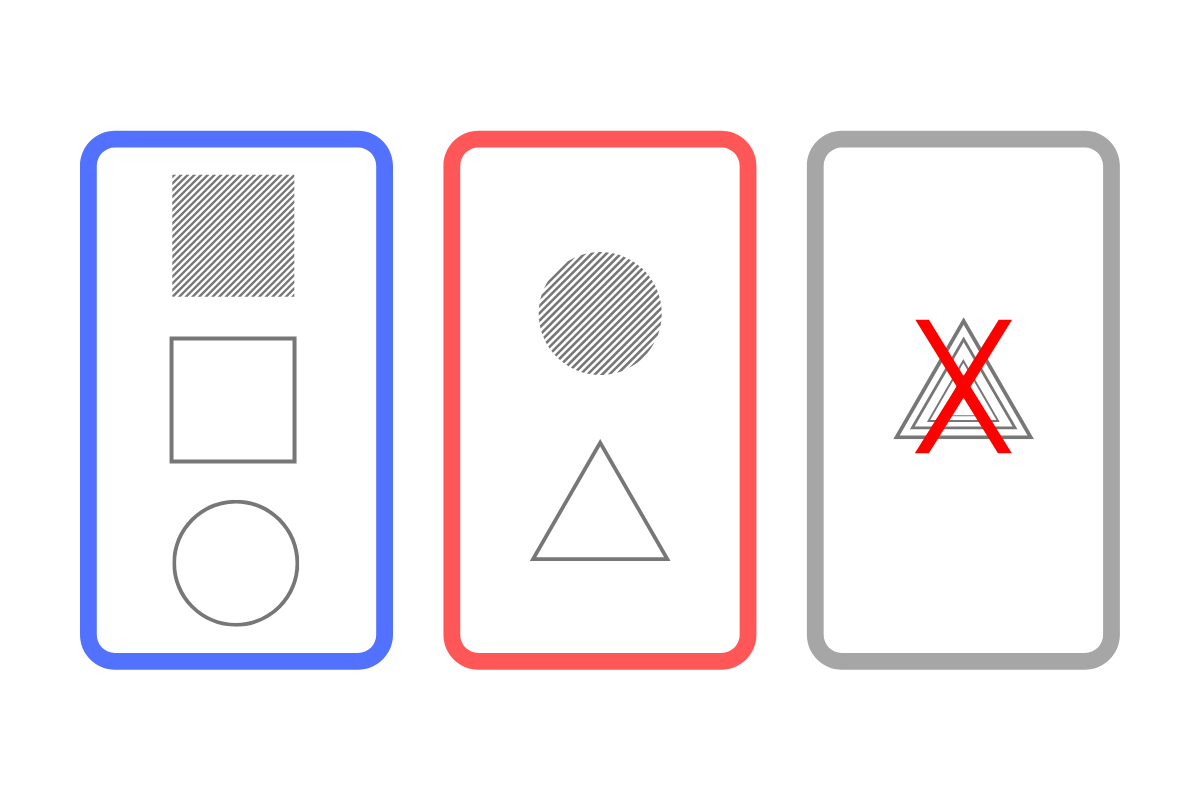
\includegraphics[width=0.45\textwidth]{Images/img1}
    \caption{Funcionamento do agente empacotador.}
    \label{fig:method}
\end{figure}
\label{example::robo}
\end{example}

\begin{example}
Agora vamos estender o exemplo \ref{example::robo} supondo que o sensor tátil não está funcionando corretamente, e ele irá sentir objetos lisos como se fossem ondulados. Para nosso exemplo, vamos considerar que o primeiro item será um triângulo liso. Nenhum erro ocorre quando a câmera percebe o triângulo, mas o sensor tátil indica que ele é ondulado. Nesse caso, teremos uma ilusão, pois triângulo é um objeto válido, mas ele foi percebido com uma propriedade inválida, que não existe no contexto do agente. Não há planos para quando o agente detecta esse tipo de erro, então ele pode executar um plano padrão para casos de erro, ou simplesmente não fazer nada.
\label{example::ilusao1}
\end{example}{}

Esse tipo de anomalia demonstrado no exemplo \ref{example::ilusao1} será chamado de ilusão classe 1, onde o corpo do predicado, ou o objeto da percepção, é válido, mas possui um argumento ou uma característica inválida.

\begin{definition}{}
   Uma ilusão classe 1 é uma percepção do tipo \texttt{objeto(caracteristica)} ou equivalente, onde \texttt{objeto} é um elemento do contexto do agente e \texttt{característica} não é.
\end{definition}

\begin{example}
    Se considerarmos que as percepções do agente possuem formas erradas por conta de um defeito na câmera ou o software de reconhecimento de padrões que atua sobre ela, um objeto como um círculo liso pode ser reconhecido como um estrela listrada. Estrela não é um objeto válido, mas listrado é.
    \label{example::ilusao2}
\end{example}{}

Isso será chamado de ilusão classe 2, definido de maneira similar a ilusão classe 1.

\begin{definition}{}
   Uma ilusão classe 2 é uma percepção do tipo \texttt{objeto(caracteristica)} ou equivalente, onde \texttt{objeto} não é um elemento do contexto do agente e \texttt{característica} é.
\end{definition}

Portanto, podemos simplesmente definir ilusão da seguinte forma:

\begin{definition}{}
   Uma ilusão é uma percepção do tipo \texttt{objeto(caracteristica)} ou equivalente, que se caracteriza como uma ilusão classe 1 ou uma ilusão classe 2.
\end{definition}

\subsection{Alucinação}

\begin{example} {}
    Retornando ao exemplo \ref{example::ilusao1} do agente responsável por empacotar os itens, mas que agora apresenta também o comportamento defeituoso do exemplo \ref{example::ilusao2}. Uma percepção formalmente correta, do tipo \texttt{objeto(caracteristica)}, por conta dos erros que os sensores possurm podem resultar na percepção \texttt{estrela(ondulada)}. Essa percepção poderia ser processada pelo agente, entretanto ela não faz parte de seu contexto, e cairia também em algum plano padrão para casos de erro ou simplesmente não executar nada.
    \label{exemple::alucinacao}
\end{example}

Assim, uma alucinação é um tipo específico de ilusão classe 1 e classe 2, podendo acarretar os mais diversos tipos de erros dentro do raciocínio do agente, ou gerando problemas caso seja ignorada. Portanto, uma alucinação pode ser definida da seguinte maneira:

\begin{definition}{}
   Uma alucinação é uma percepção do tipo \texttt{objeto(caracteristica)} ou equivalente, onde nem \texttt{objeto} nem \texttt{característica} é um elemento do contexto do agente.
\end{definition}

\section{Planejamento Automatizado}

Planejamento automatizado é um dos problemas fundamentais da inteligência artificial. As motivações para usar o planejamento automatizado são a capacidade de utilizar recursos de planejamento acessíveis e eficientes e reproduzir uma parte do processo cognitivo humano com um componente totalmente integrado de comportamento deliberativo\cite{GHALLAB20041}. A maneira clássica de realizar planejamento automatizado era considerar esse um problema de dedução lógica, onde era dado um estado inicial, ações que aferam esse estado e um conjunto de estados de objetivo, e era necessário encontrar a sequência de ações que faziam com que o ambiente saísse de um estado inicial para um estado de objetivo \cite{MADANI20035}.

Uma forma alternativa de tratar o problema de planejamento automatizado é utilizando planejamento probabilístico. Essa abordagem pode ser necessária por conta do fato de que o agente provavelmente não tem conhecimento completo do mundo ao seu redor. Kushmerick et. al. apresenta um modelo utilizando esse conceito \cite{KUSHMERICK1995239}. Outra saída para o problema do planejamento automatizado, utilizada por outros autores (e. g. \cite{Cassandra:1998:EAA:926710}, \cite{DBLP:journals/corr/abs-1105-5460}, \cite{article}), são os processos de decisão de Markov. O modelo que iremos apresentar não exige uma implementação específica de planejamento automático, ficando a cargo da implementação tomar a decisão de que caminho seguir. 

Abaixo, apresentamos a definição abstrata de planejamento automático, descrita como um modelo conceitual simples que contém os elementos principais do problema, tendo sido originalmente apresentada por Ghallab et. al. \cite{GHALLAB20041}.

\begin{definition}{}
\label{definition::autoplanning}
   % USAR MAIS TARDE PARA DEFINIR O BLOCO DE AUTOPLANEJAMENTO An automated planning block is a instance of the conceptual model of automated planning, described through the interaction between three components bellow \cite{GHALLAB20041}:
   Um modelo conceitual de planejamento automatizado é descrito como a interação entre os seguintes três componentes:
   
    \begin{itemize}
        \item Um sistema de transição de estados $\Sigma$, especificado por uma função de transição de estados $y$, de acordo com os eventos e ações que ele recebe. 
        \item Um $controlador$, que dado uma entrada de estados $s$ do sistema, fornece como saída uma ação de acordo com algum plano.
        \item Um $planejador$, que dado uma entrada de uma descrição de sistema $Z$, uma situação inicial e alguns objetivos, sintetiza um plano para o controlador a fim de alcançar o objetivo.
    \end{itemize}
    
    Um sistema de transição de estados $\Sigma$ é uma quádrupla $\Sigma = \langle S, A, E, \Gamma \rangle$, onde:
    
    \begin{itemize}
        \item $S = \{s_1, s_2, ..., s_{n}\}$ é um conjunto finito ou recursivamente enumerável de estados;
        \item $A = \{a_1, a_2, ..., a_{n}\}$ é um conjunto finito ou recursivamente enumerável de ações;
        \item $E = \{e_1, e_2, ..., e_{n}\}$ é um conjunto finito ou recursivamente enumerável de eventos; e 
        \item $\Gamma: S \times A \times E \rightarrow 2^S$ é uma função de transição de estados. 
    \end{itemize}
     
\end{definition}
%% \chapter{Trabalhos Relacionados}
\chapter{Trabalhos relacionados}

\label{chapter:relacionados}

Existem diversas abordagens para otimizar as percepções recebidas por um agente, isto é, garantir que todas as informações coletadas pelos sensores sejam utilizadas da melhor maneira possível. Diversos artigos sobre o assunto, com diferentes abordagens, são publicados todos os anos. Para definir os trabalhos relacionados apresentados nessa seção, foram utilizados diversos termos de busca, uma vez que os termos ilusão e alucinação podem não necessariamente se aplicarem às percepções da mesma maneira definida neste trabalho.

Nos mecanismos de busca Google Scholar e Scopus foram realizadas pesquisas que associam agentes inteligentes a percepções inválidas, anomalias ou ilusões e alucinações, além de termos auxiliares como aprendizado e otimização. As buscas aconteceram ao longo do desenvolvimento do trabalho, e diversas \textit{strings} de busca foram utilizadas e combinadas. Conforme encontraram-se os artigos, suas introduções foram verificadas para averiguar se o conteúdo realmente estava relacionado ao processo de revisão de percepções. Depois disso foi realizada uma leitura inicial dos trabalhos selecionados, e os quatro mais adequados foram escolhidos para um estudo mais profundo.

Os artigos apresentados nas Seções \ref{van2011} e \ref{diab2019} implementam modelos para tratar de percepções em ambientes onde é possível receber percepções que não são totalmente confiáveis, semelhante ao conceito de anomalia definido no Capítulo \ref{conceitos-fundamentais}. Os artigos das Seções \ref{pangercic2010} e \ref{kim2017} são trabalhos relacionados a outros campos de estudo de percepção, mas que precisam resolver problemas relacionados a percepções imperfeitas. A maneira como esses artigos se conectam ao modelo proposto no trabalho atual está descrita em mais detalhes nas seções seguintes.

\section{Scalable perception for BDI-agents embodied in virtual environments \cite{van2011scalable}}

\label{van2011}
Ambientes virtuais como jogos, simulações e treinamentos exigem cada vez mais complexidade dos agentes com os quais os participantes interagem. A arquitetura BDI (\textit{belief-desire-intension}) provê a complexidade necessária para que os agentes virtuais desempenhem as tarefas avançadas necessárias. Porém, agentes BDI tradicionais possuem uma interface direta com o ambiente, enquanto os agentes dos jogos normalmente possuem um conjunto de sensores limitados para realizar suas percepções. O problema é que agentes BDI não possuem um mecanismo padrão para controlar seus sensores, decidindo quais percepções receber. Dessa maneira, o agente pode facilmente ficar sobrecarregado de informação. Para resolver esse problema, os autores desse trabalho criaram um \textit{framework} que fornece habilidades sensoriais e e atenção perceptiva para agentes BDI incorporados em um ambiente virtual, funcionando como um \textit{middleware} que atua entre o modelo cognitivo do agente e o ambiente.

Nesse \textit{framework} (representado na figura \ref{fig:bdiPerceptionModel}) toda informação do ambiente é representada pelo modelo de informação chamado \textit{Environment Object Model} (Modelo de Objeto de Ambiente) ou EOM. Objetos são definidos por classes e características, e existe uma hierarquia de objetos para agregar semântica. O \textit{middleware} é dividido entre a interface física e a interface cognitiva. A função da interface física é interagir com o ambiente para formar símbolos. Para tal, o processador sensorial primeiro recebe uma lista de possíveis percepções, que respeita filtros predeterminados implementados nos sensores. Após isso, esse processador determina se o agente está interessado nas informações recebidas, através do \textit{Interest Subscription Manager} (gerenciador de inscrição de interesse). Estes símbolos são passados para o agente na foma de percepções, que alteram os objetivos do agente. Os novos objetivos, por sua vez, são repassados para o sistema de atenção, que atualiza os interesses do agente no gerenciador de inscrição de interesse. A comunicação entre a interface física e a interface cognitiva é realizada através de mensagens, e há interfaces para que o \textit{middleware} possa se comunicar com o ambiente e com o agente, de maneira a mantê-lo independente de domínio. 

\begin{figure}[h!]
    \centering
    \caption{\textit{Framework} de percepção baseado em EOM.}
    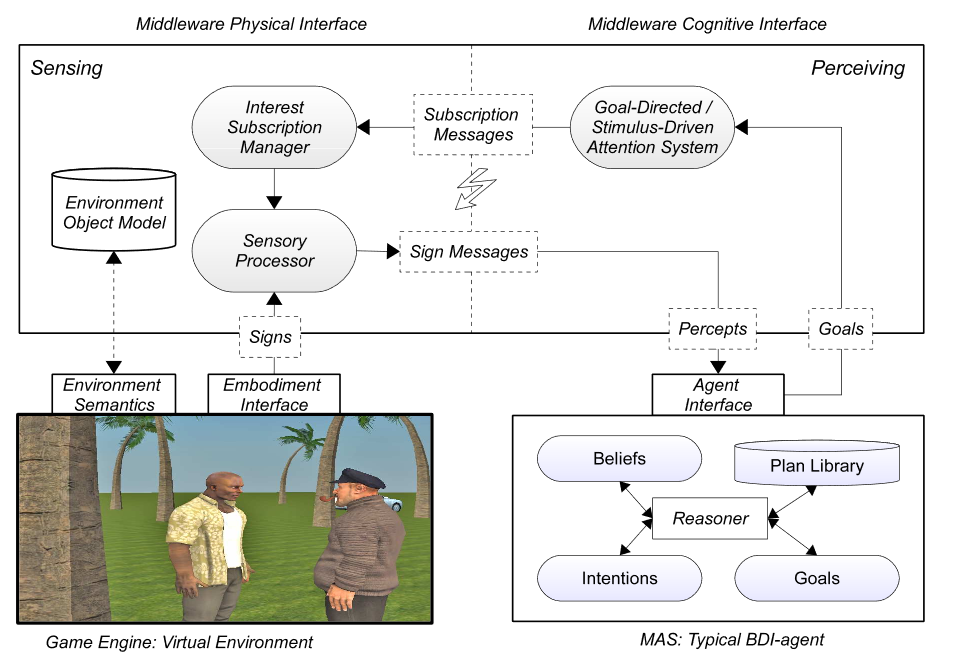
\includegraphics[width=\textwidth]{images/bdiPerceptionModel.png}
    \legend{Fonte: Scalable perception for BDI-agents embodied in virtual environments \cite{van2011scalable}.}
    \label{fig:bdiPerceptionModel}
\end{figure}

Para avaliar o modelo proposto, foram realizados dois experimentos. O primeiro consistiu no uso de sensores físicos em um teste de estresse, tanto em um sistema que utilizava o framework quando em um que não o utilizava. As percepções recebidas pelos agentes continham cinco atributos cada, sendo que a quantidade de entidades percebidas aumentava gradativamente. Cinco baterias de testes foram conduzidas para cada agente. O segundo experimento consistiu na implementação de um sistema multiagente (SMA) de agentes BDI baseado em Java e utilizando uma engine Prolog para realizar o raciocínio, e os mesmos testes do primeiro experimento foram realizados.

Esse modelo, que é capaz de decidir que tipo de percepções o agente deseja perceber de acordo com seus interesses, se assemelha ao HAIL porque muda dinamicamente ao longo do tempo, conforme as percepções são processadas. Além disso, ele possui um elemento de percepção ativa, pois o conjunto de percepções recebidas de maneira direta e massiva do ambiente é filtrado pelo processador de sensores.


\section{PMK — a knowledge processing framework for autonomous robotics perception and manipulation \cite{Diab_2019}}

\label{diab2019}
As tarefas executadas por robôs vêm se tornando cada vez mais complexas. Para realizar essas tarefas, os robôs precisam passar por uma etapa de planejamento, na qual decidem quais ações tomar baseados no estado atual do ambiente ao seu redor. Alguns dos mecanismos clássicos de planejamento utilizam a Linguagem de Definição de Domínio de Planejamento (\textit{Planning Domain Definition Language} ou PDDL) para descrever o ambiente no qual o agente está inserido. O problema é que essa abordagem assume um mundo fechado, i.e., que todos os fatos sobre o mundo são conhecidos, caso contrário o planejador pode falhar. Com essa limitação, um robô não é capaz de começar uma tarefa a não ser que todos os objetos do ambiente tenham sido reconhecidos e as ações que ele deve executar tenham sido definidas. Em outras palavras, a existência de alucinações e ilusões limita o funcionamento de tais sistemas.

Para resolver esse problema em situações onde o robô precisa realizar tarefas complexas de manipulação, foram criadas abordagens de planejamento baseadas no conhecimento, que utilizam reconhecimento semântico do cenário, conhecimento a respeito do comportamento físico de objetos e raciocínio sobre as possíveis ações de manipulação.

O trabalho de Diab et al. propõem um \textit{framework} de representação de conhecimento baseado em ontologias (uma especificação formal de conhecimento) chamado PMK (\textit{Perception and Manipulation Knowledge}), apresentado na figura \ref{fig:pmk}. Esse modelo é genérico, para que possa ser utilizado em diversos domínios, e incorporado com outras ontologias. O PMK permite associar dados de percepção de baixo nível (proveniente dos sensores, na camada física do sistema) com conhecimento de alto nível (camada de raciocínio do agente).
Uma dos principais contribuições do artigo é criar um \textit{framework} que funcione como uma caixa preta para um planejador qualquer: o PMK é capaz raciocinar sobre os recursos do robô, suas restrições de ação, a viabilidade de ação e os comportamentos de manipulação. Para isso, o modelo utiliza análise situacional, avaliando a situação a situação dos objetos no ambiente com base em posicionamento espacial, acessibilidade do robô aos objetos, potencial área na qual o objeto será colocando entre outros. 

A abordagem que é proposta pelo PMK oposta ao HAIL, pois tenta mapear todas as percepções possíveis em baixo nível a priori. Dessa forma, mesmo que o agente não tenha sido projetado para tratar determinadas percepções, ele é capaz de entender o significado semântico delas através do \textit{framework}. Em outras palavras, a ideia do PMK é criar um mapa extenso para que nenhuma percepção recebida pelo agente seja uma anomalia.

\begin{figure}
    \centering
    \caption{\textit{Framework} PMK.}
    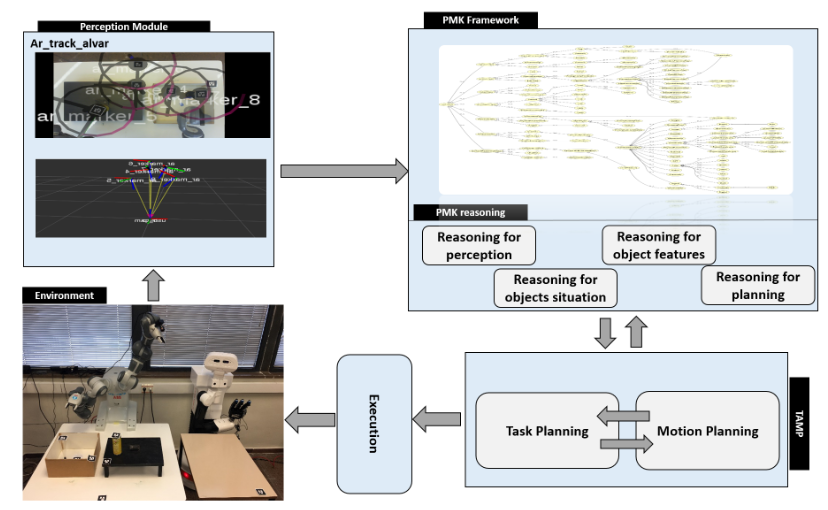
\includegraphics[width=0.9\textwidth]{images/pmk-model.png}
    \legend{Fonte: PMK - a knowledge processing framework for autonomous robotics perception and manipulation \cite{Diab_2019}.}
    \label{fig:pmk}
\end{figure}

\section{Combining perception and knowledge processing for everyday manipulation \cite{pangercic2010}}

\label{pangercic2010}
Robôs autônomos implementados para realizar tarefas de manipulação de objetos do dia a dia precisam tomar diversas decisões que requerem a combinação de percepção e processamento de conhecimento. Esse artigo de Panger et al. apresenta um sistema de programação lógica chamado K-CoPMan (\textit{Knowledge enabled Cognitive Perception for Manipulation}, ou Percepção Cognitiva Ativada pelo Conhecimento para Manipulação). Esse modelo é capaz de testar e satisfazer pré-condições de conhecimento para manipulações do dia a dia. Para isso, ele fornece ao agente o conhecimento simbólico abstrato sobre as cenas percebidas, usa conhecimento simbólico abstrato para realizar tarefas de percepção e responde a novos tipos de consultas que exigem a combinação de percepção e processamento de conhecimento.

Um dos principais mecanismos do K-CoPMan é o componente de percepção passiva. Para se tornar consciente do ambiente, o agente que utiliza tal sistema pode escanear a cena em busca de áreas de interesse, como mesas ou cadeiras, utilizar os sensores para detectar objetos. Cada objeto recebe um identificador único, para então ser guardado na base de conhecimentos, juntamente com o contexto do momento em que a percepção foi realizada. O identificador é utilizado para que mais tarde seja possível examinar mais a fundo objeto, e possivelmente classificá-lo ou categorizá-lo. Portanto, o K-CoPMan permite que agentes inteligentes estejam conscientes do ambiente ao seu redor fazendo uma varredura completa do ambiente, uma vez que utiliza tanto percepção ativa quanto passiva, e guardando as anomalias detectadas para que possam ser tratadas mais tarde por um módulo próprio (o servidor de percepção).

A abordagem desse trabalho para evitar os efeitos de percepções inválidas é similar ao PMK, mas ao invés de utilizar uma base de conhecimentos prévia para evitar que alguma percepção não possa ser tratada pelo agente, o próprio sistema cria sua base através da varredura do ambiente pela percepção passiva.

\section{Understanding human intention by connecting perception and action learning in artificial agents \cite{kim2017understanding}}

\label{kim2017}
Para desenvolver agentes capazes de realizar comportamentos complexos similares aos de seres humanos, é primeiro preciso entender como os seres humanos aprendem a perceber, pensar e agir em um mundo dinâmico. Diversos campos da inteligência artificial buscam replicar esses comportamentos, além de outros como a emoção e a cooperação. Essas habilidades parecem ser intrínsecas aos seres humanos, e tornam nossas relações mútuas únicas. Em particular, a capacidade de entender a intenção dos outros tem sido considerada a base da comunicação entre humanos. Nesse artigo, Kim, Yu e Lee propõem um modelo, chamado OA-SMTRNN (\textit{Object Augmented Supervised Multiple Timescale
Recurrent Neural Network}), para entender a intenção do usuário e responder ativamente da maneira mais adequada, através do uso de redes neurais. Para implementar o reconhecimento de intenção, são focados dois processos cognitivos, a percepção da disponibilidade de objetos e a previsão da ação humana.

Nos experimentos realizados pelos autores, diversos objetos precisaram ser percebidos pelo agente. Entretanto, alguns objetos poderiam estar sobrepostos, conforme demonstra a Figura \ref{fig:overlap}. Nesses casos, as percepções recebidas pelo agente poderiam estar incorretas. Para resolver este problema, o módulo responsável pelas ações foi implementado com a capacidade de relacionar a ação e os objetos. No artigo, é exemplificada a relação entre ``encher um copo d'água'' e ``fazer um café mocha''. Ou seja, o modelo, que foi previamente treinado, se mostrou capaz de associar a intenções como ``beber leite'' a determinadas ações (segurar um objeto, leva algo para a boca) para inferir que determinada anomalia (uma caixa de leite sobreposta por uma caneca) era uma caixa de leite.

\begin{figure}[h!]
    \centering
    \caption{Exemplo de sobreposição de imagens na percepção.}
    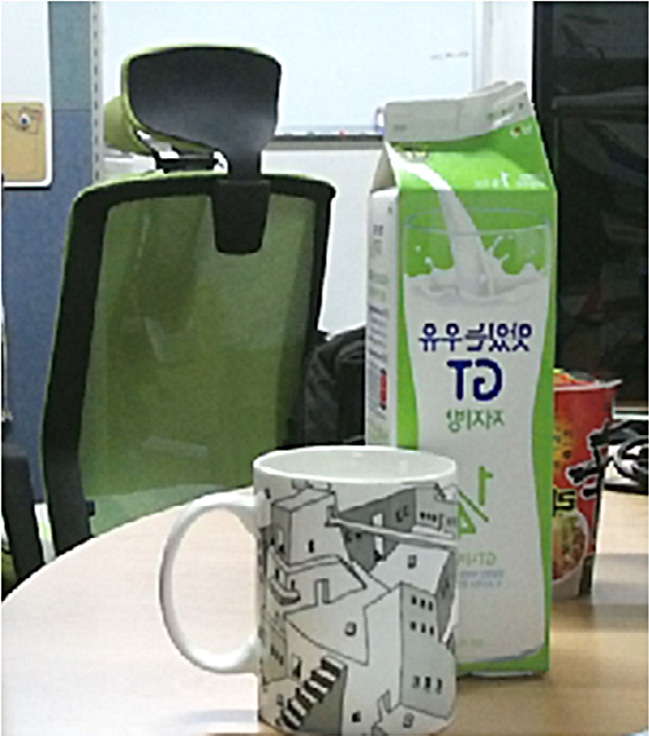
\includegraphics[width=0.5\textwidth]{images/overlap.jpg}
    \legend{Fonte: Understanding human intention by connecting perception and action learning in artificial agents \cite{kim2017understanding}.}
    \label{fig:overlap}
\end{figure}

Enquanto no modelo de revisão de percepções apresentado buscamos resolver o problema de percepção de anomalias através de uma abordagem simbólica, que classifica, trata e aprende com ilusões e alucinações, o modelo OA-SMTRNN utiliza uma abordagem conexionista, com o uso de redes neurais, para conseguir extrair semântica de percepções que seriam inicialmente inválidas para o agente. Além disso, na conclusão do trabalho é mencionado que “implementar aprendizagem de percepção-ação conectada pode desempenhar um papel importante no desenvolvimento de agentes artificiais que podem inferir a intenção humana e interagir melhor”. No HAIL, essa integração é realizada uma vez que as anomalias percebidas são utilizadas pelos módulos de planejamento automatizado para criar novos planos.

\section{Discussão}

Os quatro trabalhos que foram selecionados possuem diversas similaridades e diferenças. Para visualizar isso melhor, eles foram separados de acordo com as seguintes categorias, para então comporem o Quadro \ref{tab:relacionados}:

\begin{enumerate}
    \item Apresenta ou não um \textit{framework} genérico que pode ser aplicado em qualquer agente, independente de arquitetura;
    \item A abordagem que o trabalho utiliza para tratar percepções inválidas: limitando as percepções, de maneira que o agente realize a percepção apenas sobre as entidades que ele está pronto para tratar; definindo o ambiente, através de alguma forma de representação de conhecimento que descreve o mundo do agente para que ele possa tratar todas as percepções recebidas; ou tratar as anomalias recebidas através de algum sistema que processa as percepções inválidas recebidas;
    \item Tipos de experimentos realizados: se foram feitas simulações de software ou se foi construído um agente físico para testar o modelo;
    \item Tipos de percepções que o agente recebia: completas, no caso de ambientes simulados, ou físicas, no caso de agentes físicos;
    \item Forma de avaliação que foi utilizada para mensurar a eficácia do método proposto;
    \item Paradigma do agente (simbólico ou conexionista);
    \item Se o modelo apresenta ou não alguma ferramenta de aprendizado que utiliza ilusões e alucinações para gerar novos planos ou conhecimento.
\end{enumerate}

Através dessa classificação, é possível destacar em quais pontos nosso modelo se assemelha e diverge dos trabalhos relacionados que foram selecionados. O principal referencial do HAIL está no processo de revisão de percepções simbólico e na capacidade de permitir que qualquer arquitetura possua um processo de aprendizagem através do planejamento automatizado. Isso se reflete principalmente na forma de avaliação (tempo de processamento, como no trabalho \ref{van2011}, e também pela taxa de aprendizado do modelo) e no tipo de percepção utilizada nos experimentos (completas, pois o agente recebe a informação diretamente da simulação, mas sem semântica atrelada e sem contexto de aplicação). Além disso, três dos quatro trabalhos selecionados possuem um ambiente físico no mundo real: os trabalhos \ref{diab2019} e \ref{pangercic2010} na forma de implementação física e o trabalho \ref{kim2017} na forma de percepção de imagens que foram extraídas de um ambiente real. Isso é um indicativo de que trabalhos futuros podem implementar nosso modelo fisicamente, em robôs, por exemplo.

\begin{landscape}

% \usepackage{colortbl}


\begin{quadro}[]
\caption{Trabalhos relacionados categorizados.}
 \makegapedcells
\begin{tabular}{|P{2.3cm} |P{2.5cm}|P{2.5cm}|P{3cm}|P{2.5cm}|P{3.5cm}|P{2.3cm}|P{2.5cm}|}
\hline

\textbf{Trabalho}       & \textbf{Framework Genérico} & \textbf{Abordagem} & \textbf{Experimentos}                 & \textbf{Tipos de Percepções}                       & \textbf{Forma de Avaliação}                        & \textbf{Paradigma} & \textbf{Ferramenta de Aprendizado} \\ \hline
OIJEN; DIGNUM, 2011     & Sim (BDI)                   & Limitar percepções & Simulação de SMA com ambiente gráfico & Completas (semântica no ambiente)                  & Tempo de processamento                             & Simbólico          & Não                                \\ \hline

DIAB et al., 2019       & Sim                         & Definir o ambiente & Implementação física                  & Física (câmeras)                                   & Corretude da tarefa executada                      & Simbólico          & Não                                \\ \hline
Pangercic et. al., 2010 & Não                         & Definir o ambiente & Implementação física                  & Física (câmeras)                                   & Corretude da tarefa executada                      & Simbólico          & Não                                \\ \hline

KIM; YU; LEE, 2017      & Não                         & Tratar anomalias   & Implementação de modelo computacional & Dataset de imagens                                 & Corretude da predição                              & Conexionista       & Sim                                \\ \hline
\textbf{HAIL (trabalho atual)}          & \textbf{Sim}                         & \textbf{Tratar anomalias}   & \textbf{Simulação de agente único}             & \textbf{Completas (aleatórias e independentes de contexto)} & \textbf{Tempo de processamento e capacidade de aprendizado} & \textbf{Simbólico}          & \textbf{Sim}                                \\ \hline
\end{tabular}
 \label{tab:relacionados}
 \legend{Fonte: Autor.}
\end{quadro}

\end{landscape}


\iffalse
\newpage
\section{SEÇÃO DE TRABALHOS RELACIONADOS (ORGANIZAÇÃO)}

Essa seção estão conteúdos ligados a pesquisa de trabalhos relacionados, mas será movida ou distribuída no artigo final.

\begin{itemize}
    \item O trabalho de John Anderson [9] propõem uma versão distribuída do simulador de agentes únicos Gensim. No artigo, Anderson discorre sobre como colocar a fonte das percepções completamente dentro do agente ou do ambiente é filosoficamente impreciso. Além disso, o autor descreve como isso também representa um problema prático, uma vez que a preparação sensorial é um elemento computacionalmente intensivo, portanto um equilíbrio deve ser encontrado.
    
    \item Para Włodzisław Duch [10], em seu trabalho sobre inteligência computacional, um dos grandes problemas atuais dessa área é seu foco em raciocínio como computação, e o uso da lógica como base do raciocínio, deixando de lado o caráter técnico de como símbolos precisam primeiro serem derivados de percepções reais. Segundo o autor, o cérebro humano é altamente especializado em análise de padrões naturais e outras técnicas que permitem o mapeamento de percepções a ações, mas apesar do grande avanço na área de inteligência computacional, sistemas projetados para resolver essas funções cognitivas de ordem inferior ainda estão muito distantes da capacidade do cérebro biológico.
    
    \item Bordeux et. al. [8] apresenta uma pipeline de percepção para agentes autônomos, propondo um processo de pré-processamento, processamento e pós-processamento utilizando filtros de percepções. filtro de agente, composto por um filtro de percepção, opcionalmente um filtro semi-reflexivo (que não será discutido por estar fora do escopo do trabalho atual) e uma lista de objetos selecionados. A ideia de guardar a lista de objetos selecionados conversa com o bloco avaliador de nosso modelo, pois guarda informações de determinadas percepções realizadas para serem mais tarde reaproveitadas para um ajuste fino.
    
    \item Em um artigo de revisão sobre arquiteturas cognitivas, Langley et. al [3] caracteriza a importância de tratar de percepções imperfeitas, e mostra que as arquiteturas podem conter elementos para tratar disso, uma vez que os sensores geralmente possuem interferências ou outros tipos de ruídos, que afetam a qualidade da percepção obtida. Segundo o autor, ambientes dinâmicos complicam ainda mais a situação, uma vez que o agente precisa rastrear alterações que ocorrem muitas vezes de maneira repentina no ambiente. A única solução que o autor propõem a isso é o “conhecimento perceptivo”, onde o agente decide sobre quais sensores utilizar, onde e quando focaliza-los e que interferências são plausíveis, se aproximando da percepção ativa.
    
    \item Mesmo em simulações virtuais, às percepções podem levar a erros por conta de sua imprecisão. Sichman [6] ilustra alguns aspectos essenciais de mecanismos de raciocínio sociais, baseado na noção de dependência social. O sistema proposto trata de um modelo de coalizões, onde agentes podem se juntar em prol de um objetivo em comum. O protocolo de formação de coalizões é formado por proposições, aceitações, recusas e mensagens de revisão. As mensagens de revisão são necessárias pois uma possível razão para um agente se recusar a participar de uma coalizão é porque o remetente tem uma crença falsa sobre suas capacidades, ou seja, acreditar que o agente pode executar uma ação, mas na realidade não pode. Isso pode acontecer pois fontes de informação, como as percepções, podem levar a erros.

    \item O trabalho de Pangercic et. al. [7] trata de percepção e processamento de conhecimento, usando como estudo de caso um robô encarregado de determinar quais objetos faltam em uma mesa durante uma refeição, através de inferências lógicas. A implementação resulta em um modelo estatístico, em que cada objeto que o robô conhece recebe uma porcentagem de chance de ser necessário. Apesar dessa alta volatilidade, os autores não tratam da possibilidade da inferência incorreta.
    
    \item Diab et. al. apresenta um framework de processamento de conhecimento para a manipulação de percepção de robôs autônomos, através de raciocínio de percepção, isto é, raciocínio relacionado às características perceptivas dos objetos no ambiente, como outros modelos também fazem, mas além disso adiciona raciocínio relacionado aos algoritmos que o sensor pode executar para extrair os recursos, aos sensores associados ao robô e as limitações físicas dos sensores. Segundo os autores, esse processo torna o robô mais inteligente e flexível. Essa flexibilidade pode ser útil para lidar com a falhas de um sensores, fornecendo alternativas, ou seja, o framework proposto tem flexibilidade para lidar com sistemas sensoriais de vários modelos.
    
\end{itemize}

\textbf{Problema abordado no artigo:} Conforme abordado pelo artigo [3], interferências ocorrem entre o processo físico de percepção e o processamento final dela, dentro do ciclo cognitivo do agente. Portanto, esse trabalho ataca essa lacuna que existe, com o objetivo de minimizar percepções incorretas ou falhas completas de percepção.

\textbf{Contribuição do artigo:} Nesse artigo é apresentado um modelo genérico para o tratamento de percepções, com o objetivo de evitar que informação potencialmente útil seja desperdiçada, criando novos planos quando o agente não está pronto para lidar com percepções que estão fora do seu planejamento inicial. Esse modelo foi construído para que possa ser acoplado a qualquer arquitetura cognitiva, independente do grau de abstração que ela implemente.

\textbf{fim da seção de organização dos trabalhos relacionados}
\fi
%%\chapter{Modelo de Revisão de Percepções}

\noindent O modelo proposto para revisão de percepção é separado em três etapas, como mostra a figura \ref{fig:method}. Primeiro, o agente recebe um conjunto de percepções $p$ através de seus sensores. Depois disso, essas percepções passam através de uma função de refinamento, onde as percepções $p$ são refinadas tornando-se um subconjunto próprio $\rho$ de percepções refinadas. O conjunto $\rho$ é então passado para o módulo de alucinação e ilusão, onde cada percepção refinada passa por um processo de detecção de anomalia. As percepções de $\rho$ que forem consideradas válidas, irão constituir o subconjunto próprio $\varrho$ de percepções válidas, enquanto as anomalias formarão o subconjunto próprio $\sigma$ de anomalias. As percepções válidas são enviadas direto para o ciclo de raciocínio do agente, enquanto as anomalias irão cair em uma lista ordenada, onde aguardarão para passarem por um processo de planejamento automatizado.

Para ajudar a compreender o funcionamento desse modelo integrado ao raciocínio de um agente, nós usaremos uma versão estendida do exemplo \ref{example::robo}, um pouco mais complexa para podermos demonstrar passo a passo como funciona o modelo. 

\begin{example}
    Partindo do exemplo \ref{example::robo}, vamos supor que agora a loja vende estrelas lisas e listrados, que podem ser empacotadas com qualquer um dos pacotes. Além disso, o mesmo robô responsável por empacotar os itens que passavam por uma esteira é responsável por empacotar itens de três diferentes esteiras. As percepções são as mesmas que antes, mas agora ele é capaz de perceber os itens nas três esteiras, através de novos sensores táteis e de uma câmera que capta uma imagem aberta o suficiente para isso. As percepções continuam sendo do tipo \texttt{forma(textura)}.
    \label{example::robo2}
\end{example}{}

\begin{figure}[h!]
    \centering
    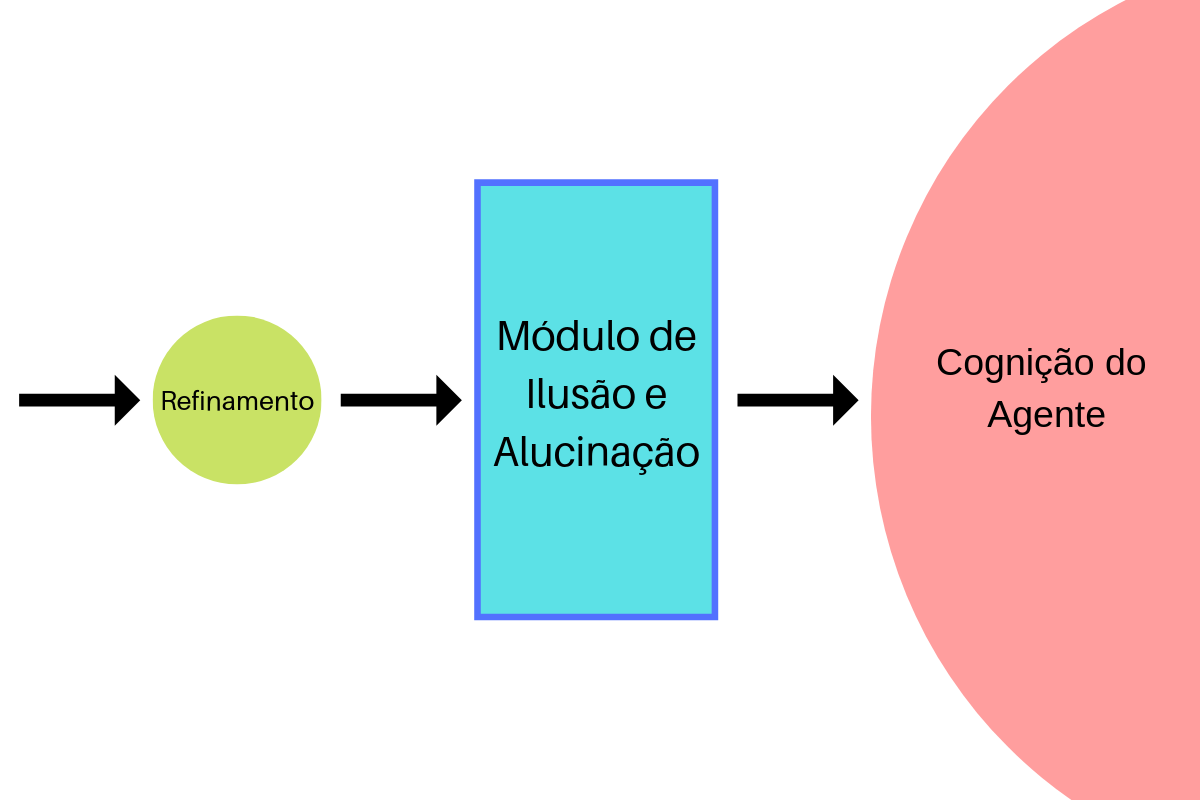
\includegraphics[width=0.8\textwidth]{Images/img2.png}
    \caption{Modelo de revisão de percepções.}
    \label{fig:method}
\end{figure}

\section{Módulo de refinamento}

O módulo de refinamento serve como uma primeira filtro para que percepções indesejadas pelo agente não cheguem até seu ciclo de raciocínio. O processo de refinamento é descrito pela definição \ref{def:refinamento}.

Caso não seja de interesse de uma determina arquitetura ou implementação de uma arquitetura refinar suas percepções, como pode ser o caso de um sistema especialista, o módulo de percepção pode simplesmente ter uma função tal que $f(x) = x$, com as percepções passando por dentro sem nenhum processo, possuindo assim o subconjunto próprio $\rho = p$.

\begin{example}
    Continuando o exemplo \ref{example::robo2}, as estrelas não fazem parte da área de atuação desse robô, e portanto para otimizarmos o processo de empacotamento é possível utilizar o módulo de percepções para refinar a informação recebida pelos sensores para enviar menos informações desnecessárias para a cognição do agente. Nesse exemplo, o robô pode ser implementado com uma função $\theta$ que realiza percepção ativa, removendo assim as percepções que não fazem sentido dentro do contexto em que ele está inserido. O conjunto de percepções $p$ passa pelo processo de percepção ativa e devolve $\rho$, que tem nesse caso específico, sendo $s$ o conjunto de percepções possíveis envolvendo estrelas, um comportamento tal que o conjunto $p$ sob a operação $\theta$ retorna $\rho = p \cap \overline{s}$. 
    Para tornar o processo mais tangível, vamos supor que o agente recebe o conjunto $p_i$ de percepções, composto por $\{circle(stripped), triangle(smooth), star(yellow)\}$. A operação $\theta$ vai remover de $p_i$ os elementos contidos no conjunto $s$ de possíveis percepções envolvendo estrelas, conforme foi descrito anteriormente. Portanto, a saída do bloco de percepções será $\rho = \{cicle(stripped), triangle(smooth)\}$.
    
\end{example}{}

\section{Módulo de Alucinação e Ilusão}

\begin{figure}[h]
    \centering
    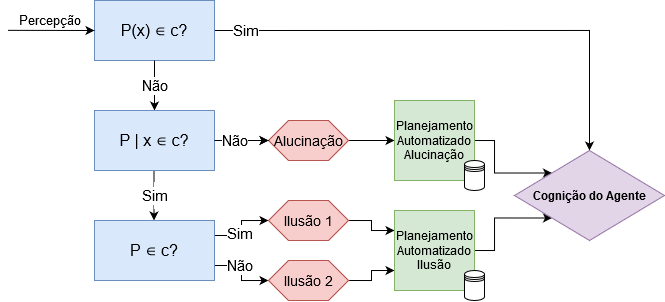
\includegraphics[width=0.8\textwidth]{Images/diagrama-modelo.png}
    \caption{Módulo de alucinação e ilusão.}
    \label{fig:model}
\end{figure}
 
 A figura \ref{fig:model} é a representação gráfica do módulo de alucinação e ilusão, que começa com a entrada $\rho$ sendo dirigida para o decisor 1. O primeiro decisor responde a pergunta: ``A percepção recebida está no código do agente?''. Caso a resposta for sim, consideramos a percepção como válida, e ela é enviada para a cognição do agente. Caso a resposta seja não, consideramos $\rho(x)$ uma anomalia, e enviamos ela para o segundo decisor, que responde a pergunta: ``O corpo ou o argumento do predicado $\rho(x)$ se encontra em alguma parte do código?''. Caso a resposta seja não, concluímos que a anomalia é uma alucinação. Caso contrário, ela é considerada uma ilusão e é enviada para o terceiro decisor. O terceiro decisor responde a pergunta: ``O corpo do predicado $\rho(x)$ está no código?''. Caso a resposta for sim, a ilusão é considerada uma ilusão classe 1, caso contrário, é considerado uma ilusão classe 2. Toda essa cadeia de decisores é representada pelo algoritmo abaixo:

\begin{algorithm}[H]
\SetKwInOut{Input}{input}
\Input{agent context \textit{c}, perception $\rho(x)$}

  \uIf{$\rho(x)$ is in \textit{c}}{
   $\rho(x)$ is a valid perception\;
   }\uElseIf{neither $\rho$ nor $x$ is in c}{
   $\rho(x)$ is a hallucination\;
   }\uElseIf{$\rho$ is in \texttt{c}}{
   $\rho(x)$ is an illusion class 1\;
  }\Else{$\rho(x)$ is an illusion class 2}
 \label{algorithm:decisor}
 \caption{Funcionamento dos decisores do módulo de ilusão e alucinação}
 \label{alg::selection}
\end{algorithm}

\begin{example}
    Para entender como as percepções são tratadas pelos decisores, vamos supor algumas entradas possíveis para o exemplo \ref{example::robo2}, que terão diferentes comportamentos ao longo do tempo de execução do nosso exemplo. Primeiro, vamos supor o caso mais básico, em que o agente recebe a percepção \texttt{quadrado(riscado)}. Essa é uma percepção completamente válida dentro do contexto do agente, pois ele possui um plano específico para tratar dessa percepção, que é empacotar o objeto com o papel vermelho. Portanto, nesse caso, $p(x) = \rho(x)$. Após sair do módulo de percepções, $\rho(x)$ passa como entrada para o decisor 1, que detecta que existe um plano específico para tratar da entrada, portanto a percepção é considerada válida e é diretamente enviada para a cognição do agente.

    Caso uma percepção não seja válida, ela é enviada para os decisores subsequentes, para que a anomalia seja devidamente classificada. 
\end{example}{}

\subsection{Bloco Avaliador}

Após a classificação da anomalia, ela é enviada para um bloco avaliador, que tratará de decidir qual anomalia pode ser considerada relevante para ocupar o planejamento automatizado e quais podem simplesmente retornar para o módulo de percepção para ajudar no processo de refinamento.
O funcionamento de um bloco avaliador deve permitir que alucinações ou ilusões seja processadas quando há tempo de processamento ocioso e o contexto permite. Para isso, vamos utilizar uma espécie de escalonador combinado com uma lista ponderada. Vamos considerar o tempo $c_m(\rho)$ o tempo médio de processamento gasto para cada percepção do conjunto $\rho$ recebido pelo agente, $a_m(\rho)$ o tempo médio do processamento das anomalias do conjunto $\rho$ recebida por um bloco de planejamento automatizado e $l_a$ a lista ponderada de $a$, onde $a$ é o índice que representa um dos três blocos avaliadores (de alucinação, ilusão classe 1 ou ilusão classe 2) utilizado para manter a generalidade. O principio do funcionamento da fila ponderada é o mesmo de uma fila comum, First in First Out (FIFO). Quando um elemento é inserido pela primeira vez na fila, ele recebe o peso 1. Quando uma cópia do mesmo elemento é inserida novamente, o elemento tem seu peso adicionado em 1, como mostra a figura \ref{filaPonderada}. Além disso, sendo $\rho$ o conjunto de percepções recebido pelo bloco de alucinação e ilusão, $|\rho|$ o número de percepções do conjunto e $\rho_a$ o número de anomalias.

O bloco avaliador seleciona quando uma percepção deve ser tratada através de uma função matemática, levando em conta o tempo médio de processamento de uma percepção válida e de uma anomalia, através da função de processamento. Além desse funcionamento básico, o bloco avaliador ainda contém um mecanismo para remover anomalias classificadas com irrelevantes para o sistema, através de uma função de limpeza. Caso essa função retorne verdadeiro, todos os elementos de peso 1 da sua respectiva lista são removidos. Essas duas funções serão trabalhadas na seção de formalismo.

\begin{figure}[h!]
    \centering
    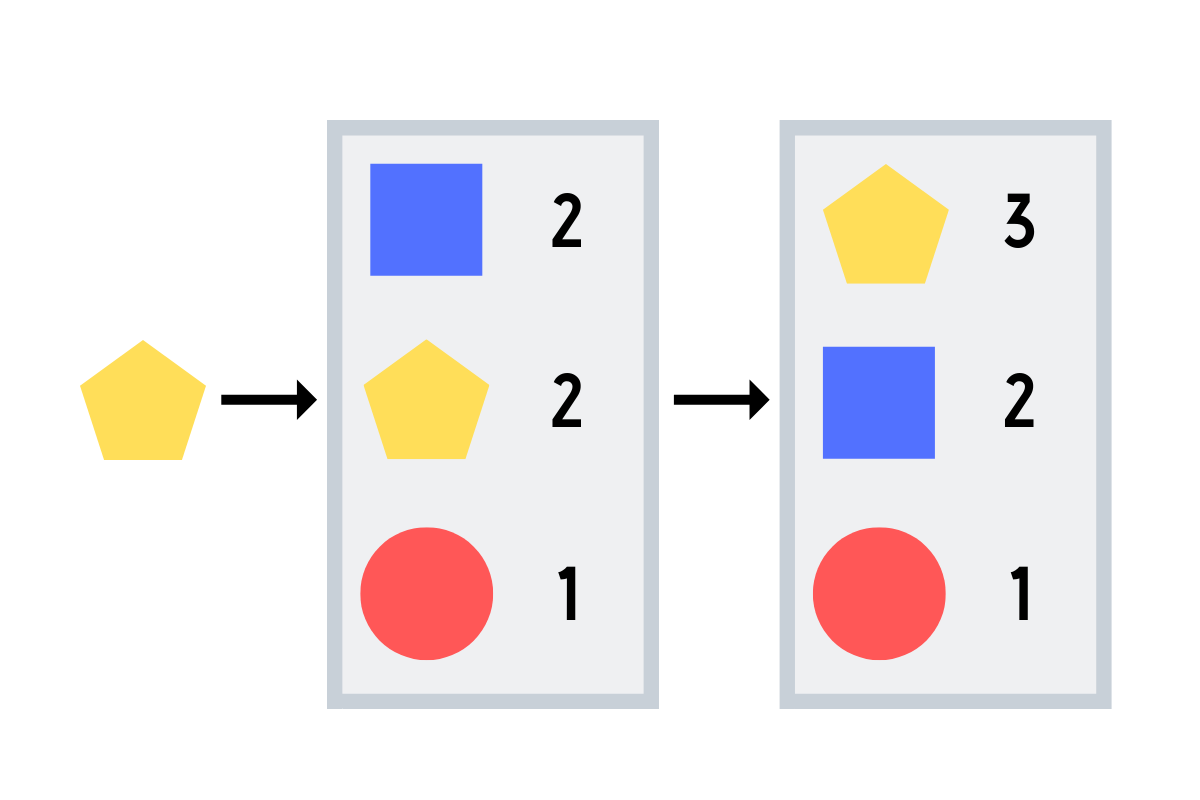
\includegraphics[width=0.49\textwidth]{Images/filaPonderada.png}
    \caption{Exemplo de fila ponderada.}
    \label{filaPonderada}
\end{figure}

\begin{example}
    Vamos supor que a percepção recebida pelo agente foi \texttt{lua(serrilhada)}. Lua não é um item que deveria ser percebido pelo agente, mas ou a implementação da percepção ativa foi simplória demais, simplesmente filtrando as estrelas, ou houve alguma falha que permitiu que ela chegasse ao módulo de alucinação e ilusão. Uma das propostas do modelo é detectar esse tipo de anomalia, que é uma falha completa do sistema. Quando ela chega ao decisor 1, é classificada como anomalia, pois não faz parte do escopo do agente. Em seguida, a percepção é enviada para o decisor 2, que verifica que não existe nenhuma menção de nenhuma parte da percepção no comportamento do robô, ou seja, é uma alucinação. Uma vez detectada a alucinação, a percepção segue para o bloco avaliador, onde será inserida na fila ponderada com o peso 1. Como consideramos apenas uma percepção recebida, e essa percepção é considerada uma anomalia, a equação da função de processamento é validada, e a anomalia segue para o bloco de planejamento automatizado.
\end{example}{}

\subsection{Bloco de Planejamento Automatizado}

O bloco de planejamento automatizado é potencialmente a parte mais custosa computacionalmente, e a parte mais difícil de ser implementada por todo o sistema. Um planejamento automatizado puramente simbólico tende a ser extremamente pesado, uma vez que pode considerar milhares de alternativas para o estado de mundo atual, tentando chegar mais perto de seu objetivo. Um processo de planejamento automatizado conexionista é uma opção, já que estamos tratando de uma análise incompleta do mundo, tratando do desconhecido. Teorias mais rebuscadas como criatividade computacional\cite{colton2012computational} podem ser adicionadas aqui, criando mais uma camada de complexidade para o agente, mas em troca dando um resultado ainda mais preciso para a avaliação da qualidade da percepção.

Uma percepção pode chegar ao bloco de planejamento automatizado quando ela for a primeira na fila ponderada e a função de processamento retornar verdadeiro. De um ciclo para outro, as percepções permanecem na fila, a não ser que sejam descartadas pelo mecanismo de limpeza. Nosso modelo não explicita qual é a ordem que os blocos avaliadores devem processar suas filas para mandar anomalias para o planejamento automatizado, ficando a cargo da implementação em questão tomar essa decisão.


\begin{example}
    Para mostrar o caminho que faz uma ilusão, vamos considerar que o agente recebe em duas esteiras a percepção \texttt{triangulo(listrado)}. Não existem triângulos listrados na loja, mas como $\theta$ não filtra essa percepção, ela vai chegar ao decisor 1. Como não existe um plano específico para tratar essa percepção, ela é considerada uma anomalia, e é encaminhada ao decisor 2. Como existe um plano para tratar de triângulos lisos, a percepção é então classificada como uma ilusão, e vai para o terceiro decisor. Nele, como o plano trata triângulos, a percepção é considerada uma ilusão classe 1. Finalmente após a percepção ter sido classificada corretamente, ela é enviada para o bloco avaliador, e é inserida na fila ponderada com peso 1. Depois disso, a percepção da segunda esteira, que é igual a que já foi tratada, chega ao bloco de alucinação e ilusão. Essa percepção vai fazer o mesmo caminho até o bloco avaliador e o peso da anomalia já presente na fila é aumentada para 2. Como duas percepções foram consideradas anomalias, vamos considerar que a função de processamento seja satisfeita, e o bloco avaliador passa essa anomalia para o bloco de planejamento automatizado.
    
    Após uma percepção ser considerada relevante para ser enviada ao planejamento automatizado, ela deve gerar um novo plano para aquela percepção a ser adicionada ao conjunto de planos do agente, e essa percepção então deixará de ser uma anomalia. Ilusões e alucinações tem blocos de planejamento automatizado separados para permitir que duas implementações completamente diferentes sejam utilizadas de acordo com a função do agente e a necessidade de criar novos planos eficientes. Retomando o exemplo dois, quando o planejamento automatizado de alucinações recebe a percepção \texttt{lua(serrilhada)}, um processo de planejamento automatizado deve ser executado. Para esse exemplo, consideremos um planejamento automatizado puramente simbólico, que analisa uma grande quantidade de estados futuros possíveis para o ambiente em que o robô está inserido e seleciona aquele que será mais eficiente para que o agente se aproxime de seu objetivo principal (terminar de empacotar os itens). Isso é extremamente custoso, mas como alucinações são muito raras para esse agente em questão, pois ele já tenta eliminar ao máximo percepções fora de seu escopo através da percepção ativa. Portanto, é um custo que vale a pena pois vai gerar um plano eficiente, evitando novas alucinações. No exemplo, é possível que a lua seja resultado de um corte errado na peça circular. Portanto, o agente precisa descartar esse item, para evitar gasto com embalagem desnecessária e que o item seja repassada para uma próxima etapa, gerando ainda mais custo. Assim, um novo plano da forma \texttt{lua(serrilhada) -> descartar} é adicionado, e \texttt{lua(serrilhada)} deixa de ser uma alucinação.

    No caso da percepção \texttt{triângulo(listrado)} do segundo exemplo, o agente poderia ter um bloco de planejamento automatizado baseado em uma rede baysiana, uma vez que ilusões podem ser muito mais comuns e o agente já tem uma breve noção do que deve ser feita com objetos do tipo. \texttt{triângulo(listrado)} pode ser um novo item a venda na loja, e como já foi verificado em duas esteiras diferentes, faz sentido que ele não seja uma mera falha de sensores. Assim, o planejamento automatizado pode inferir o plano \texttt{triângulo(listrado) -> empacotar}, permitindo que o agente tenha um aprendizado dinâmico resultado da adição de um novo plano em seu conjunto de planos. Assim como no caso da ilusão, uma vez que esse plano novo foi adicionado a percepção original deixa de ser uma anomalia, uma vez que faz parte do contexto em que o agente está trabalhando.

\end{example}{}

%% \chapter{Implementação e Simulação}
\chapter{Material e Métodos}

A partir da construção do modelo proposto no capítulo anterior, a próxima etapa foi a sua formalização. Após termos um modelo formal, construímos um pseudocódigo que pode ser implementado em qualquer linguagem de programação. Para validar o modelo, foi feita uma implementação genéria (sem arquitetura cognitiva) em Python, apresentada no próximo capítulo).

\section{Formalização}

A formalização foi realizada em um modelo de cascata, onde se começa com uma única tupla, que se desdobra para conceitos mais complexos e específicos. O objetivo disso é criar camadas de abstração, sobre as quais podem ser criadas variações de acordo com a necessidade de implementações específicas ou da integração com arquiteturas cognitivas.

 O bloco básico do modelo proposto, chamado de \emph{Modelo de Revisão de Percepções}, é composto por duas unidades: (i) um módulo para alucinação e ilusão $M_{ih}$; (ii) uma função de refinamento $\theta$. O módulo de ilusão e alucinação é uma quádrupla, apresentada na definição \ref{def:illuHallu}. A função de refinamento é uma função abstrata, cuja entrada é obtida através dos sensores do agentes e a saída é a entrada do módulo de alucinação e ilusão. Ela recebe um conjunto de percepções qualquer $p$ e retorna um subconjunto próprio $\rho$, ou seja, é uma função que pode ou não reduzir o número de percepções que são enviadas ao modulo de ilusão e alucinação.

\begin{definition}{}
    Um modelo de revisão de percepções é uma dupla $R = \langle M_{ih}, \theta \rangle$, onde:
    
    \begin{itemize}
        \item $M_{ih}$ é o bloco de ilusão e alucinação; e
        \item $\theta$ é a função de refinamento $\theta(p) = \rho$, onde $p$ é um conjunto de percepções e $\rho$ é um subconjunto próprio de $p$.
    \end{itemize}{}
    
\end{definition}

Após ter passado pela função $\theta$, as percepções $\rho$ irão passar pelo algoritmo \ref{alg::selection}, descrito por uma quádrupla, com conjuntos de decisores e blocos e uma função de transição.

\begin{definition}
\label{def:illuHallu}
    O bloco de alucinação e ilusão é uma quádrupla $M_{ih} = \langle D, Ab, Ap, \Delta \rangle$, onde:
    
    \begin{itemize}
        \item $D$ é o conjunto de decisores $D = \{d_{a}, d_{h}, d_{i}\}$, onde:
             \begin{itemize}
                \item $d_{a}$ é o decisor de anomalias, descrito pela função:
                \[ d_{a} = \left\{ \begin{array}{ll}
                0 & \mbox{se $\rho(x)$ está em $c$ \footnotemark};\\
                1 & \mbox{se $\rho(x)$ não está em $c$}.\end{array} \right. \]
             
                \item $d_{h}$ é o decisor de alucinação, descrito pela função:
                \[ d_{h} = \left\{ \begin{array}{ll}
                0 & \mbox{se nem $\rho$ nem $(x)$ está em $c$};\\
                1 & \mbox{se $\rho$ ou $(x)$ está em $c$}.\end{array} \right. \]
                
                \item $d_{i}$ é o decisor de ilusão, definido pela função:
                \[ d_{i} = \left\{ \begin{array}{ll}
                0 & \mbox{se $\rho$ está em $c$};\\
                1 & \mbox{se $(x)$ está em $c$}.\end{array} \right. \]
            \end{itemize}
        
        \footnotetext{ $c$ é o contexto do agente, de acordo com a definição \ref{definition::context}.}
        
        \item $Ab$ é o conjunto de blocos avaliadores $Ab = \{Ab_{h}, Ab_{i1}, Ab_{i2}\}$, onde $Ab_{h}$ é o bloco de avaliação de alucinações, $Ab_{i1}$ é o bloco de avaliação de ilusões classe 1 e $Ab_{i2}$ é o bloco de avaliação de ilusões classe 2.
        
        \item $Ap$ é o conjunto de blocos de planejamento automatizado $Ap = \{Ap_{h}, Ap_{i}\}$, onde $Ap_{h}$ é o bloco de planejamento automatizado de alucinações e $Ap_{i}$ é o bloco de planejamento automatizado de ilusões.
        
        \item $\Delta$ é a função de transição definido pela tabela abaixo, onde $out$ é um estado final, que leva a percepção para fora do modelo de revisão de percepções, ou seja, pode ser tanto uma transição para descartar a percepção quanto para levá-la para o ciclo de raciocínio do agente como uma percepção válida.
        
            \begin{table}[htb]
                \centering
                \begin{tabular}{c c c c} 
                    \toprule
                    \textbf{State} & \textbf{0} & \textbf{1} \\
                    \midrule
                    $d_{a}$     & $out$     & $d_{h}$       \\
                    $d_{h}$     & $Ab_{h}$  & $d_{i}$       \\
                    $d_{i}$     & $Ab_{i1}$ & $Ab_{i2}$     \\
                    $Ab_{h}$    & $out$     & $Ap_{h}$      \\
                    $Ab_{i1}$   & $out$     & $Ap_{i}$      \\
                    $Ab_{i2}$   & $out$     & $Ap_{i}$      \\
                    \bottomrule
                \end{tabular}
                \label{transition-table}
                \caption{Tabela de transição $\Delta$ do módulo de ilusão e alucinação}
                
            \end{table}
    \end{itemize}{}
\end{definition}{}

O módulo de alucinação e ilusão é o corpo principal do modelo. Ele recebe uma entrada $\rho$, que é a saída da função de refinamento apresentada na definição 1, e processa cada um dos elementos $\rho(x)$ desse conjunto, através de decisores e blocos de avaliação, percorrendo o modelo de acordo com as transições descritas pela função de transição $\Delta$. Os três decisores do conjunto $D$ fazem a triagem para detectar se a percepção $\rho(x)$ é uma anomalia, e que tipo de anomalia é. Após passar pelos três decisores, saberemos se essa percepção é valida, é uma alucinação, é uma ilusão tipo 1 ou uma ilusão tipo 2.

Após ter passado pelos decisores, a percepção fica armazenada nos blocos avaliadores, que serão descritos posteriormente, onde por fim poderá ser descartada ou enviada para um módulo de planejamento automatizado.

\begin{definition}
    Um bloco avaliador é uma tripla $Ab_{x} = \langle L, Pf, Cf) \rangle$, $x \in \{h, i1, i2\}$, onde:

    \begin{itemize}
        \item $L$ é uma lista ordenada pelo número de vezes que uma mesma anomalia é dada como entrada;
        \item $Pf$ é a função de processamento, definida abaixo:
            
             \[ Pf = \left\{ \begin{array}{ll}
                        1 & \mbox{if $T_{m}(A) \leq T_{m}(V) * (|A| - |A_{pr}|)$;}\\
                        0 & \mbox{caso contrário}.\end{array} \right. \]
        
            
            Onde:
            
            \begin{itemize}
                \item $T_{m}$ é a função que retorna a média do tempo gasto para processar as percepções de um conjunto;
                \item $A$ é o conjunto de anomalias, $A(x)$ é um elemento específico $x$ e $|A|$ o número de anomalias do conjunto;
                \item $A_{pr}$ é o conjunto de anomalias que já foram validades para serem processadas pela função de processamento neste ciclo de raciocínio ($A_{pr}$ é instanciada vazia a cada ciclo de raciocínio), e $|A_{pr}|$ o número de anomalias desse conjunto.
                \item $V$ é o conjunto de percepções válidas.
            \end{itemize}{}
        
        \item $Cf$ é a função de limpeza conforme definida abaixo, sendo $\alpha$ um coeficiente variável que precisa ser definido pela instância do modelo de revisão de percepções:
        
        \[ Cf = \left\{ \begin{array}{ll}
                        1 & \mbox{se  $Ce = Verdadeiro$;}\\
                        0 & \mbox{caso contrário}.\end{array} \right. \]
            
            \[ Ce = \sum_{i=1}^{|L|} P_{n}(L_{i}) > \alpha \sum_{j=1}^{|L|} P_{1}(L_{j}) \]
            
            Onde:
            
            \begin{itemize}
                \item $L$ é a lista ordenada do bloco, sendo $|L|$ o número de anomalias únicas e $L_{i}$ a anomalia $i$ da lista.
                \item $P$ é a função $P(L_{i}) = |L_{i}|$, sendo $|L_{i}|$ o peso da anomalia especificada (número de entradas recebidas dessa mesma anomalia na lista). A função $P$ é utilizada para especificar as seguintes funções:
                \\
                
                    (i) $ P_{1}(L_{i}) = \left\{ \begin{array}{ll}
                        1 & \mbox{se $P(L_{i}) = 1$;}\\
                        0 & \mbox{caso contrário}.\end{array} \right. $
                \\
                
                    (ii) $ P_{n}(L_{i}) = \left\{ \begin{array}{ll}
                        P(L{i}) & \mbox{se $P(L_{i}) > 1$;}\\
                        0 & \mbox{caso contrário}.\end{array} \right. $
            \end{itemize}{}
    \end{itemize}
\end{definition}{}

A terceira definição é a de bloco de avaliação ($Ab$). Um $Ab$ é um módulo do modelo que é responsável por armazenar as anomalias detectadas e decidir se elas serão processadas pelo agente ou não. É descrito por uma tripla, constituída por uma lista ordenada $L$, uma função de processamento $Pf$ e uma função de limpeza $Cf$. $L$ é uma lista organizada pela recorrência de elementos inseridos nela, onde cada elemento só aparece uma vez e contém um número de vezes que o mesmo elemento já foi inserido nela, chamado de peso. Nesse modelo, os elementos são as anomalias percebidas pelo agente, e o peso é o número de vezes que o agente percebeu a anomalia.

$Pf$ é uma função que avalia se uma anomalia será processada nesse ciclo de raciocínio ou se será armazenada para ser processada no futuro. Para isso, ela precisa de uma função que retorne o tempo médio previsto para o processamento de uma percepção $T_m$, seja ela uma percepção válida ou uma anomalia. Com base nessa função, $Pf$ retorna 1 caso o tempo médio de processamento de uma anomalia seja menor que o tempo médio de processamento de uma percepção válida multiplicado pelo número de anomalias que fazem parte desse ciclo de raciocínio menos o número de anomalias que já foram aprovadas pelo bloco avaliador, e zero caso contrário.

De maneira simplificada, o que essa função busca evitar que o modelo de revisão de percepção gaste mais tempo de processamento do que ele gastaria caso não estivesse sendo utilizado, processando apenas as anomalias que aparecem de maneira mais recorrente para o agente.

$Cf$ é uma função que realiza a limpeza de $L$. Conforme os ciclos de raciocínio forem passando, $L$ tende a possuir diversas anomalias que foram percebidas apenas uma única vez. Dessa maneira, uma grande quantidade de memória seria necessária para armazenar as possíveis centenas de anomalias que podem nunca ser processadas. Assim, a função $Cf$ verifica se a equação $Ce$ é verdadeira ou falsa. Ela é verdadeira quando o número de anomalias que apareceram uma única vez é maior que a soma dos pesos das anomalias que apareceram mais de uma vez (o peso é o número atrelado a cada anomalia, que representa quantas vezes elas já foram inseridas na linha). Quando a função for verdadeira, o bloco avaliador remove todas as anomalias de peso 1 da lista.

\begin{definition}
    Um bloco de planejamento automatizado é uma instância do modelo conceitual de planejamento automatizado (definição \ref{definition::autoplanning}).
\end{definition}

\section{Pseudocódigo}

O pseudocódigo apresentado nessa seção é um esqueleto na qual implementações reais do modelo proposto possam se basear. A sequência de comandos apresentada deve ser aplicada entre o momento que a percepção é recebida pelo agente e a efetiva entrada da percepção no seu ciclo de raciocínio.

\begin{algorithm}[h]
\While{True}{
    $p \leftarrow$ sensors.percept\\
    $\rho \leftarrow \theta(p)$\\
    
    $c \leftarrow$ agent.getContext\\
    
    \ForEach{perception $\rho(x)$ in $\rho$}{
        decide $\rho(x)$ perception type based on $c$\\
        \If{$\rho(x)$ is hallucination}{\\
            $Ab_{h} \leftarrow \rho(x)$ \\
            $A \leftarrow \rho(x)$\\ 
        }
        \ElseIf{$\rho(x)$ is illusion class 1}{
            $Ab_{i1} \leftarrow \rho(x)$ \\
            $A \leftarrow \rho(x)$\\ 
        }
        \ElseIf{$\rho(x)$ is illusion class 2}{
            $Ab_{i2} \leftarrow \rho(x)$ \\
            $A \leftarrow \rho(x)$\\ 
        }
        \Else{
            $V \leftarrow \rho(x)$\\ 
        }
        
    }
    x $\leftarrow$ choose(i1, i2, h)\\
        
        \While{$Ab_x$ == True}{
            $t \leftarrow$ top of $Ab_x$'s L
            $plan \leftarrow Ap_{x}$.autoplan($t$)\\
            add $plan$ to P\\
            add $t$ to $A_{pr}$\\
        }
        \ForEach{y in (i1, i2, h)}{
            \If{$Ab_{y}.Cf$ == True}{
                clean $Ab_x$'s L
            }
        }
    }
    \caption{Algoritmo de avaliação de percepções}
    \label{algorithm:model}
\end{algorithm}

Para facilitar a compreensão do algoritmo, iremos explicá-lo linha a linha.

Colocamos o algoritmo dentro de um \emph{while true} para representar a continuidade do algoritmo, que executa todo ciclo de raciocínio. Nas linhas 2 e 3, o agente recebe as percepções através dos sensores, e aplica elas na função de refinamento $\theta$. Na linha 4, colocamos o contexto do agente na variável c. Isso é necessário pois sempre que esse algoritmo executa, é possível que o contexto mude, uma vez que novas percepções e planos passam pelo processo de cognição. Na linha 6, a percepção passa pelo processo de classificação, descrito em detalhes no algoritmo \ref{algorithm:decisor}. Entre a linha 7 e 21, caso a percepção seja uma anomalia, ela é adicionada ao bloco avaliador corresponde, e também ao conjunto de anomalias. Caso seja uma percepção válida, é apenas adicionada ao conjunto de percepções validas. Na linha 23, é realizado um processo de escolha de qual tipo de anomalia será tratada nesse ciclo de raciocínio. Essa escolha pode ser aleatória ou utilizar qualquer tipo de métrica escolhida pelo programador ao implementar o modelo. O tipo escolhido é avaliado na linha 24, onde o laço de repetição \emph{while} irá manter o planejamento automatizado recebendo o topo da lista ponderada enquanto a função de processamento permitir. Quando uma percepção é enviada ao planejamento automatizado, ela é adicionada ao conjunto de anomalias processadas. Nesse trecho de código foi realizado uma simplificação, pois não existe $Ap_{i1}$ e $Ap_{i2}$, apenas $Ap_{i}$, mas consideramos isso algo a ser tratado na implementação. Por fim, entre a linha 29 e a 33 é verificado se cada uma das listas ponderadas precisa ser limpa, utilizando a função de limpeza.

%% \chapter{Simulação e Resultados}
\chapter{Resultados e Discussão}

Para analisar as capacidades do modelo proposto, foram realizados três experimentos. Os dois primeiros experimentos foram implementados utilizando o design $2^k$ fatorial \cite{jain1990art}. Esse tipo de design consiste em variar $k$ fatores em 2 níveis diferentes, -1 e 1, que são extremos opostos. Por exemplo, em uma pesquisa ligada a um processador, um fator pode ser o número de núcleos, e seus níveis serem 1 núcleo e 8 núcleos. Portanto, o fator é uma variável livre, que é utilizada para analisar a variação de uma variável dependente qualquer. Os fatores e as variáveis livres utilizadas estão nas tabelas \ref{table:experiments_factors} e \ref{table:experiments_variables}, respectivamente. A análise do impacto dos fatores foi realizada utilizando a equação de regressão não linear do design $2^k$ fatorial. 
%O código implementado para essa análise está disponível no anexo [NÚMERO].

\begin{table}[h!]
    \begin{center}
        \caption{ Fatores utilizados nos experimentos. }
        \label{table:experiments_factors}
        \begin{tabular}{|c|c|c|c|}
        \hline
        \textbf{Fatores} & \textbf{Sigla} & \textbf{Nível -1} & \textbf{Nível 1} \\
        \hline
        Porcentagem de Percepções Inválidas & PPI & 5\% & 95\%  \\
        \hline
        Tempo Médio Gasto Pelo Autoplanejamento & TMA & 1/2 CR & 64 CR \\
        \hline
        Tempo Médio Gasto em um Ciclo de Raciocínio & TMC & 01 CR & 32 CR \\
        \hline
        Número de Percepções Recebidas por Ciclo & NPC & 01 & 16 \\
        \hline
    \end{tabular}{}
    \end{center}
\end{table}{}

\begin{table}[h!]
    \begin{center}
        \caption{ Variáveis dependentes analisadas nos experimentos. }
        \label{table:experiments_variables}
        \begin{tabularx}{\textwidth}{ |Y|Y| }
            \hline
            \textbf{Variáveis} & \textbf{Justificativa} \\
            \hline
            Tempo Virtual Decorrido & Medir desempenho geral do modelo \\
            \hline
            Planos Criados & Avaliar potencial do modelo de inserir aprendizado em arquiteturas que não o possuem \\
            \hline
            Percepções Processadas & Analisar a capacidade do modelo de ganhar desempenho ao longo do tempo\\
            \hline
        \end{tabularx}{}
    \end{center}{}
\end{table}

As simulações consistem na execução do modelo proposto, que foi implementado em Python, submetido a um grande volume de percepções. O agente utilizado na simulação segue os exemplos apresentados no capítulo 4 (robô embrulhador).
Uma simulação possui 5000 ciclos, sendo que cada ciclo pode possuir uma ou várias percepções. Essas percepções podem ser válidas (pertencentes ao contexto do agente) ou inválidas (não pertencentes ao contexto do agente), sendo que a proporção entre o tipo de percepções é definido pela PPI. As percepções são produzidas aleatoriamente por um gerador de percepções. As percepções válidas são geradas sorteando percepções que pertencem ao contexto do agente, e as percepções inválidas são geradas utilizando o pacote \texttt{RandomWords} \cite{pipRandomWords}. Cada ciclo da simulação segue os seguintes passos:

\begin{enumerate}
    \item Gerar as percepções da simulação;
    \item Iterar sobre cada um dos ciclos, passando as percepções para o modelo implementado;
    \item Salvar os resultados, o agente final (com novos planos gerados pelo módulo de planejamento automatizado) e as percepções de cada ciclo em arquivos CSV.
\end{enumerate}

\begin{figure}[h!]
    \centering
    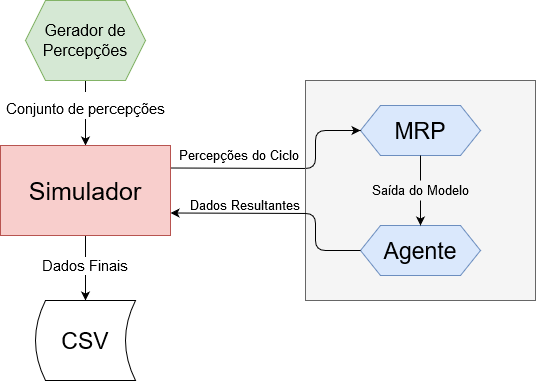
\includegraphics[width=0.8\textwidth]{Images/diagrama-simulacao.png}
    \caption{Diagrama da execução de uma iteração de cada experimento.}
    \label{fig:diagrama-simulacao}
\end{figure}

Além da configuração dos valores dos fatores, é possível configurar se um agente será recarregado (ou seja, se ele deve manter os planos gerados por uma simulação anterior) e se o simulador deve gerar novas percepções ou não, pulando a etapa 1 de cada ciclo.

Como é um experimento feito para uma arquitetura cognitiva genérica, vamos supor que o tempo de processamento que o agente gasta em cada ciclo de raciocínio é constante, e o tempo gasto pelo módulo de planejamento automatizado será calculado em função desse valor, ou seja, se o tempo do ciclo de raciocínio é o mesmo do planejamento automatizado, vamos dizer que o tempo do planejamento automatizado é 1 CR (ciclo de raciocínio).

\section{Experimento 1}

O objetivo do primeiro experimento é analisar a variação no tempo do ciclo de raciocínio e a quantidade de planos criados pelo módulo de planejamento automatizado, de acordo variações nos quatro fatores apresentados. Cada simulação foi repetida dez vezes, para que uma média pudesse ser obtida. Apesar do uso de repetições, não foi usada a metodologia do design $2^k r$ fatorial, que considera as possíveis falhas referente as repetições, pois o resíduo dos experimentos é extremamente baixo, da ordem de grandeza de $e^{-12}$.

\subsection{Resultados}

A média dos resultados de cada simulação estão apresentados na tabela \ref{table:experimento1.}. Os valor final do tempo virtual decorrido varia bastante, principalmente nas simulações com alto nível de percepções inválidas. Em dois momentos o tempo virtual foi 5000. Isso ocorreu pois nessas simulações o TMC é 1, o TMA é 0.5 e o NPC é 16. Portanto, ciclos de percepções válidas consumiam 1 unidade de tempo (4750). O bloco avaliados sempre permitia o processamento de 2 percepções inválidas (pois cada uma toma 0.5 unidades de tempo), e quase sempre há percepções inválidas disponíveis na fila pois entram 16 percepções inválidas por ciclo de percepções inválidas. Portanto, cada vez que o modelo processava percepções inválidas, ele consumia 1 unidade de tempo, e isso aconteceu 250 vezes (5\% de 5000).

\begin{table}[h!]
    \begin{center}
        \caption{ Resultados do experimento 1}
        \label{table:experimento1}
        \begin{tabular}{ |c|c|c|c|c|c|c| }
            \hline
            \textbf{Simulação} & \textbf{PPI} & \textbf{TMC} & \textbf{TMA} & \textbf{NPC} & \textbf{Tempo Virtual} & \textbf{Planos Criados}\\
            \hline
            1 & 5\% & 1 & 1/2 & 1 & 4874.6 & 250.8\\
            \hline
            2 & 5\% & 1 & 1/2 & 16 & 5000.0 & 502.0\\
            \hline
            3 & 5\% & 1 & 64 & 1 & 20806.7 & 250.9\\
            \hline
            4 & 5\% & 1 & 64 & 16 & 20813.0 & 251.0\\
            \hline
            5 & 5\% & 32 & 1/2 & 1 & 152093.5 & 251.0\\
            \hline
            6 & 5\% & 32 & 1/2 & 16 & 153437.3 & 2932.2\\
            \hline
            7 & 5\% & 32 & 64 & 1 & 168028.8 & 250.9\\
            \hline
            8 & 5\% & 32 & 64 & 16 & 168032.0 & 251.0\\
            \hline
            9 & 95\% & 1 & 1/2 & 1 & 3229.2 & 3541.6\\
            \hline
            10 & 95\% & 1 & 1/2 & 16 & 5000.00 & 9303.8\\
            \hline
            11 & 95\% & 1 & 64 & 1 & 228668.9 & 3550.3\\
            \hline
            12 & 95\% & 1 & 64 & 16 & 304300.4 & 4750.8\\
            \hline
            13 & 95\% & 32 & 1/2 & 1 & 48521.5 & 3539.0\\
            \hline
            14 & 95\% & 32 & 1/2 & 16 & 140683.3 & 4073.8\\
            \hline
            15 & 95\% & 32 & 64 & 1 & 273609.6 & 3550.3\\
            \hline
            16 & 95\% & 32 & 64 & 16 & 312032.0 & 4751.0\\
            \hline
        \end{tabular}{}
    \end{center}{}
\end{table}

O número de planos criados se agruparam em certos conjuntos de valores, de acordo com os níveis dos fatores. Como esperado, as simulações com menor porcentagem de percepções inválidas criaram menos planos, pois houveram menos anomalias, logo menos material para o módulo de planejamento automatizado trabalhar. O gráfico da figura \ref{fig:pc_occurrences} mostra a ocorrência dos resultados em certos valores aproximados.

\begin{figure}[h!]
    \centering
    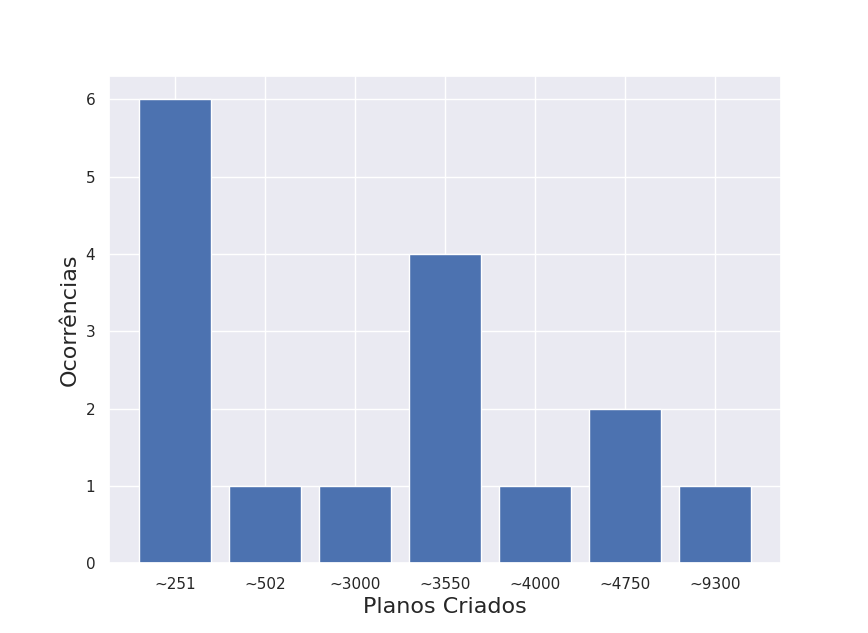
\includegraphics[width=0.8\textwidth]{Images/plans_created_occurrences.png}
    \caption{Recorrência do valor final de Planos Criados nas simulações realizadas.}
    \label{fig:pc_occurrences}
\end{figure}

\subsection{Análise de Fatores}

Conforme mostra a tabela \ref{tab:experimento1fatores}, na variável dependente de Tempo Virtual, os fatores TMC e TMA isolados tiveram uma alta porcentagem de impacto. Isso porque a contagem do tempo virtual acontecia em função justamente dos eventos de realizar planejamento automatizado e executar um ciclo de raciocínio. Portanto, a interferência nesses fatores influencia diretamente o resultado final. Além disso, a combinação dos fatores PPI + TMA teve um impacto bastante grande, de 24.13\%. Isoladamente, PPI e TMA possuem porcentagens altas (12.69 e 31.64, respectivamente), portanto era esperado que a sua
combinação também tivesse uma porcentagem alta. Entretanto, TMC possui 22.20 porcento de impacto, mas a combinação PPI + TMC possui apenas 4.16. Isso demonstra como uma combinação de alta taxa de percepções inválidas com um tempo de planejamento automatizado alto podem ser impactantes no resultado de um agente que executa o modelo.

\begin{table}
    \begin{center}
        \caption{Análise dos fatores do experimento 1}
        \label{tab:experimento1fatores}
        \begin{tabular}{ |c|c|c| }
            \hline
            \textbf{Fator} & \textbf{Efeito Tempo Virtual} & \textbf{Efeito Planos Criados}\\  
            \hline
            PPI & 12.69\% & 66.10\%\\
            \hline
            TMC & 22.20\% & 0.50\%\\
            \hline
            TMA & 31.64\% & 2.95\%\\
            \hline
            NPC & 1.44\% & 8.67\%\\
            \hline
            PPI + TMC & 4.16\% & 3.76\%\\
            \hline
            PPI + TMA & 24.13\% & 0.05\%\\
            \hline
            PPI + NPC & 1.39\% & 2.13\%\\
            \hline
            TMC + TMA & 0.55\% & 0.50\%\\
            \hline
            TMC + NPC & 0.10\% & 0.50\%\\
            \hline
            TMA + NPC & 0.01\% & 2.99\%\\
            \hline
            PPI + TMC + TMA & 0.53\% & 3.76\%\\
            \hline
            PPI + TMC + NPC & 0.09\% & 3.75\%\\
            \hline
            PPI + TMA + NPC & 0.02\% & 0.06\%\\
            \hline
            TMC + TMA + NPC & 0.54\% & 0.50\%\\
            \hline
            PPI + TMC + TMA + NPC & 0.52\% & 3.76\%\\
            \hline
        \end{tabular}{}
    \end{center}{}
\end{table}


Na variável dependente Planos Criados, a fator que mais impactou o resultado foi o PPI. Isso era o esperado, pois quanto mais percepções inválidas o modelo recebe, mais planos podem ser criados. Os outros fatores tiveram impactos bem mais baixos. O NPC teve 8.67\% de influência pois simulações com mais percepções inválidas por ciclo preenchem a fila ponderada mais rápido, sempre tendo combustível para alimentar o bloco de planejamento automatizado.

%%%%%%%%%%%%%%%%%%%%%%%%%%%%%%%%%%%%%%%%%%%%%%%%%%%%%%%%%%%%%%%%%%%%

\section{Simulação 2}

A segunda simulação foi realizada para analisar o ganho de performance de um agente ao aplicar os planos criados com o bloco de autoplanejamento. Esse segundo experimento segue os moldes do primeiro, porém foi realizado apenas uma iteração para cada configuração de fatores, e após ser realizado uma simulação com uma dada configuração, foi realizada uma nova simulação com os mesmos fatores, mas usando o agente resultante da primeira. Assim, os planos criados pelo agente foram reaproveitados.

Essa simulação pode ter sua configuração de fatores separadas em dois grupos: (I) o tempo de processamento de um ciclo de raciocínio é menor do que o tempo do autopĺanejamento; (II) o tempo do autoplanejamento é menor que o tempo de processamento de um ciclo de raciocínio. Essa separação pode ser feita pois quanto mais planos criados temos, menos percepções inválidas serão recebidas pelo agente. Portanto, se o tempo de processamento de um ciclo for maior que o de autoplanejamento, o tempo virtual gasto total usando um agente que já aprendeu vários planos será maior. Isso é um \textit{trade off} pois agora essas novas
percepções (que eram antes anomalias) estão efetivamente sendo utilizadas pelo agente.

\subsection{Resultados}

Os resultados estão separados em tabelas por variável dependente e por grupo, como descrito anteriormente. As tabelas contém o índice da simulação, os níveis dos fatores, os resultados da primeira e da segunda iteração (R1 e R2, respectivamente) e a relação percentual entre os resultados, ou seja, a proporção de R2 em relação a R1, obtido através do cálculo $(R2 * 100) / R1$.

Em todas as tabelas, podem ser observadas um menor efeito na relação percentual nas simulações que utilizaram o nível $-1$ do fator PPI (5\% de percepções inválidas). Isso se dá ao fato do menor impacto do modelo em ambientes de baixo volume de percepções inválidas, uma vez que o modelo apenas age quando há percepções inválidas na fila ponderada.

Na tabela \ref{table:vtaltv1}, a média da relação percentual foi de 75.26\%, se destacando a simulação 5 com uma relação percentual de 4.77\%. Com o tempo de autoplanejamento alto, tempo de processamento de um ciclo de raciocínio baixo e apenas uma percepção por ciclo, é notável o ganho de desempenho. Um comportamento similar (porém invertido) pode ser observado na tabela \ref{table:vtaltv2}, cuja média da relação percentual foi de 136.33\%. Nessas simulações, o esperado era que o tempo virtual subisse conforme a quantidade de planos criados aumentasse, resultando nesse comportamento similar porém invertido, conforma explicado anteriormente. 

\begin{table}
    \begin{center}
        \caption{ Alteração do Tempo Virtual no Grupo I }
        \label{table:vtaltv1}
        \begin{tabular}{ |c|c|c|c|c|c|c|c| }
            \hline
            \textbf{Simulação} & \textbf{PPI} & \textbf{TMC} & \textbf{TMA} & \textbf{NPC} & \textbf{R1} & \textbf{R2} & \textbf{Relação Percentual}\\
            \hline
            1.1 & 5\% & 1 & 64 & 1 & 20750.0 & 20687.0 & 99.70\%\\
            \hline
            1.2 & 5\% & 1 & 64 & 16 & 20813.0 & 20750.0 & 99.70\%\\
            \hline
            1.3 & 5\% & 32 & 64 & 1 & 168032.0 & 167968.0 & 99.96\%\\
            \hline
            1.4 & 5\% & 32 & 64 & 16 & 168032.0 & 168000.0 & 99.98\%\\
            \hline
            1.5 & 95\% & 1 & 64 & 1 & 227579.0 & 10859.0 & 4.77\%\\
            \hline
            1.6 & 95\% & 1 & 64 & 16 & 304313.0 & 177998.0 & 58.49\%\\
            \hline
            1.7 & 95\% & 32 & 64 & 1 & 273536.0 & 162400.0 & 59.37\%\\
            \hline
            1.8 & 95\% & 32 & 64 & 16 & 312032.0 & 250048.0 & 80.14\%\\
            \hline
            
        \end{tabular}{}
    \end{center}{}
\end{table}

\begin{table}
    \begin{center}
        \caption{ Alteração do Tempo Virtual no Grupo II }
        \label{table:vtaltv2}
        \begin{tabular}{ |c|c|c|c|c|c|c|c| }
            \hline
            \textbf{Simulação} & \textbf{PPI} & \textbf{TMC} & \textbf{TMA} & \textbf{NPC} & \textbf{R1} & \textbf{R2} & \textbf{Ganho Percentual}\\
            \hline
            2.1 & 5\% & 1 & 1/2 & 1 & 4874.5 & 4876.5 & 100.04\%\\
            \hline
            2.2 & 5\% & 1 & 1/2 & 16 & 5000.0 & 5000.0 & 100\%\\
            \hline
            2.3 & 5\% & 32 & 1/2 & 1 & 152093.5 & 152219.5 & 100.08\%\\
            \hline
            2.4 & 5\% & 32 & 1/2 & 16 & 153435.5 & 152887.0 & 99.64\%\\
            \hline
            2.5 & 95\% & 1 & 1/2 & 1 & 3228.5 & 4955.0 & 153.48\%\\
            \hline
            2.6 & 95\% & 1 & 1/2 & 16 & 5000.00 & 4944.0 & 98.88\%\\
            \hline
            2.7 & 95\% & 32 & 1/2 & 1 & 48458.5 & 157385.5 & 324.78\%\\
            \hline
            2.8 & 95\% & 32 & 1/2 & 16 & 160000.0 & 140631.0 & 113.77\%\\
            \hline
            
        \end{tabular}{}
    \end{center}{}
\end{table}

Apesar do aumento do tempo virtual das simulação, pode ser usado uma terceira variável, a quantidade de percepções válidas processadas, para analizar o desempenho do modelo. Isso porque de uma simulação para outra, o sistema de autoplanejamento armazena novos planos, e mesmo que o tempo virtual aumente, o agente está sendo capaz de processar mais informação. A média de percepções válidas processadas nas primeiras simulações de cada configuração de fatores foi de 30563.0625 percepções, enquanto nas segundas simulações foi de 40599.75, totalizando um ganho aproximado de 32.84\% de desempenho para essa variável.

As tabelas \ref{table:plansaltv1} e \ref{table:plansaltv2} mostram a variação do ganho de planos criados entre as simulações. Ambas apresentam uma queda drástica nessa variável nas simulações com 95\% de percepções inválidas, pois foram nessas simulações que o modelo pode criar mais planos (pois o autoplanejamento é utilizado mais vezes). As simulações 1.6 e 1.8 possuem um resultado acima das
simulações 1.5 e 1.7, apesar das quatro possuírem PPI de 95\%, pois possuem mais percepções (16 vezes mais, pois são 16 percepções por ciclo) e processam apenas uma percepção inválida por ciclo (pois o TMA é maior que o TMC).
A tabela \ref{table:plansaltv2} em especial possui valores ainda menores na relação percentual pois muitas percepções inválidas são processadas por ciclo, em especial na simulação 2.8, onde nenhum plano novo foi criado na segunda simulação.

\begin{table}
    \begin{center}
        \caption{ Alteração nos Planos Criados no Grupo I }
        \label{table:plansaltv1}
        \begin{tabular}{ |c|c|c|c|c|c|c|c| }
            \hline
            \textbf{Simulação} & \textbf{PPI} & \textbf{TMC} & \textbf{TMA} & \textbf{NPC} & \textbf{R1} & \textbf{R2} & \textbf{Relação Percentual}\\
            \hline
            1.1 & 5\% & 1 & 64 & 1 & 250.0 & 249.0 & 99.60\%\\
            \hline
            1.2 & 5\% & 1 & 64 & 16 & 251.0 & 250.0 & 99.60\%\\
            \hline
            1.3 & 5\% & 32 & 64 & 1 & 251.0 & 249.0 & 99.20\%\\
            \hline
            1.4 & 5\% & 32 & 64 & 16 & 251.0 & 250.0 & 99.60\%\\
            \hline
            1.5 & 95\% & 1 & 64 & 1 & 3533.0 & 93.0 & 2.63\%\\
            \hline
            1.6 & 95\% & 1 & 64 & 16 & 4751.0 & 2746.0 & 57.80\%\\
            \hline
            1.7 & 95\% & 32 & 64 & 1 & 3548.0 & 75.0 & 2.11\%\\
            \hline
            1.8 & 95\% & 32 & 64 & 16 & 4751.0 & 2814.0 & 59.23\%\\
            \hline
            
        \end{tabular}{}
    \end{center}{}
\end{table}


\begin{table}
    \begin{center}
        \caption{ Alteração nos Planos Criados no Grupo II }
        \label{table:plansaltv2}
        \begin{tabular}{ |c|c|c|c|c|c|c|c| }
            \hline
            \textbf{Simulação} & \textbf{PPI} & \textbf{TMC} & \textbf{TMA} & \textbf{NPC} & \textbf{R1} & \textbf{R2} & \textbf{Ganho Percentual}\\
            \hline
            2.1 & 5\% & 1 & 1/2 & 1 & 251.0 & 247.0 & 98.41\%\\
            \hline
            2.2 & 5\% & 1 & 1/2 & 16 & 502.0 & 500.0 & 99.60\%\\
            \hline
            2.3 & 5\% & 32 & 1/2 & 1 & 251.0 & 247.0 & 98.41\%\\
            \hline
            2.4 & 5\% & 32 & 1/2 & 16 & 2935.0 & 878.0 & 29.91\%\\
            \hline
            2.5 & 95\% & 1 & 1/2 & 1 & 3543.0 & 90.0 & 2.54\%\\
            \hline
            2.6 & 95\% & 1 & 1/2 & 16 & 9312.0 & 260.0 & 2.79\%\\
            \hline
            2.7 & 95\% & 32 & 1/2 & 1 & 3541.0 & 83.0 & 2.34\%\\
            \hline
            2.8 & 95\% & 32 & 1/2 & 16 & 4078.0 & 0.0 & 0.0\%\\
            \hline
            
        \end{tabular}{}
    \end{center}{}
\end{table}

\section{Simulação 3}

O objetivo da simulação 3 é observar a capacidade de aprendizado do agente ao longo do tempo. Para isso, foram executadas 5 simulações com os mesmos fatores (como demonstra a tabela \ref{table:experiment3factors}), mas entre uma simulação e outra o agente não foi recarregado, ou seja, manteve o aprendizado das simulações anteriores. As percepções foram geradas de maneira igual aos experimentos anteriores.

\begin{table}[h!]
    \begin{center}
        \caption{ Valor dos fatores no experimento 3. }
        \label{table:experiment3factors}
        \begin{tabular}{ |c|c| }
            \hline
            \textbf{Fator} & \textbf{Valor}\\
            \hline
            PPI & 50\%\\
            \hline
            TMC & 16\\
            \hline
            TMA & 32\\
            \hline
            NPC & 8\\
            \hline
        \end{tabular}{}
    \end{center}{}
\end{table}

Os resultados estão expostos na tabela \ref{table:experiment3results}. Nela, pode-se notar o comportamento dos três fatores observados. Enquanto os planos criados diminuem a cada simulação, pois menos percepções são inválidas (uma vez que o agente aprende com as simulações anteriores), a quantidade de percepções válidas processadas aumenta. Esse comportamento é demonstrado na figura \ref{fig:perceptions_v_plans-experiment3}. Além disso, o tempo virtual cai na mesma proporção que os planos criados diminuem, uma vez que a criação de um plano é duas vezes mais custosa em tempo do que o processamento de uma percepção válida.

\begin{table}
    \begin{center}
        \caption{ Resultados obtidos no experimento 3. }
        \label{table:experiment3results}
        \begin{tabular}{ |c|c|c|c| }
            \hline
            \textbf{Simulação} & \textbf{Planos Criados} & \textbf{Percepções Válidas Processadas} & \textbf{Tempo Virtual}\\
            \hline
            1 & 2501 & 21788 & 120016 \\
            \hline
            2 & 2454 & 30558 & 119264 \\
            \hline
            3 & 946 & 38641 & 95136 \\
            \hline
            4 & 40 & 39959 & 80640 \\
            \hline
            5 & 0 & 40000 & 80000 \\
            \hline
        \end{tabular}{}
    \end{center}{}
\end{table}



\begin{figure}
    \centering
    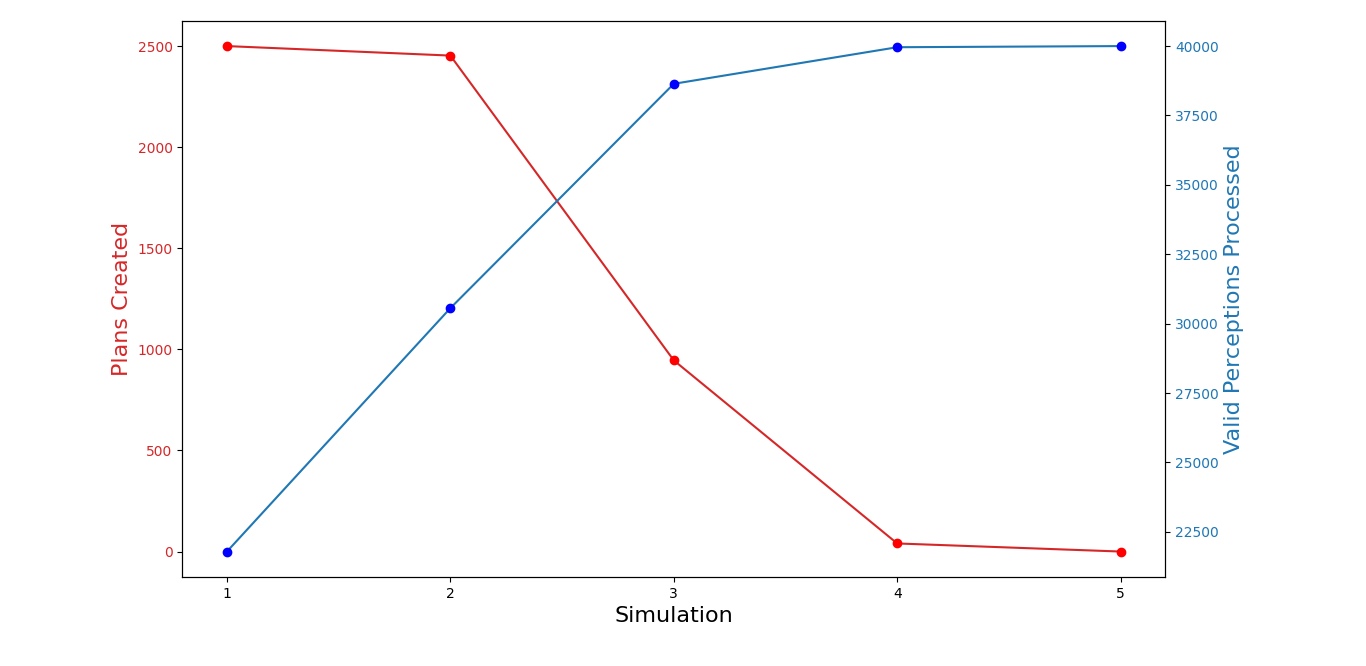
\includegraphics[width=\textwidth]{Images/perceptions_vs_plans.png}
    \caption{Evolução das percepções válidas processadas e dos planos novos criados ao longo das simulações}
    \label{fig:perceptions_v_plans-experiment3}
\end{figure}
%\chapter{Conclusão}

Neste trabalho, foi apresentado um modelo de revisão de percepções. Tal modelo, inspirado pelos conceitos de alucinação e ilusão, é capaz de reduzir as percepções recebidas, detectar percepções anômalas (que fogem do escopo de trabalho do agente), classificá-las de acordo com suas características como ilusão (do tipo 1 ou 2, conforme definido) ou alucinação e tratá-las, através do mecanismo de autoplanejamento.

O funcionamento do modelo foi descrito no capítulo 3, e sua formalização e implementação apresentadas no capítulo 4. Os experimentos realizados demonstram que o funcionamento do modelo é como esperado, sendo capaz de absorver as anomalias recebidas do ambiente e melhorar o comportamento do agente baseado nelas. Os resultados dos experimentos foram apresentados no capítulo 5. 
Analisando os resultados, é possível observar que o modelo funciona melhor em cenários onde há uma grande quantidade de percepções anômalas, possibilitando uma maior criação de planos novos. Além disso, o maior desafio do modelo é manter o desempenho do agente em cenários onde o tempo gasto pelo módulo de autoplanejamento é muito elevado.

Apesar dos experimentos terem resultados positivos, as simulações estavam limitadas a um cenário sem escopo, ou seja, sem objetivo no mundo real. Por conta disso, quase não haviam fatores aleatórios, tornando a análise extremamente precisa (com erros da ordem de grandeza de $e^{-12}$) mas também bastante limitada.
Portanto, é necessário ainda validar o modelo em mais três etapas: (i) acoplando-o a uma arquitetura cognitiva implementada, para verificar como ela se comporta em uma interação mais complexa com o ambiente; (ii) implementação de experimentos mais complexos, com simulações de alguma situação real que possa ter resultados mais palpáveis; (iii) a aplicação do modelo em agentes físicos, para verificar se ele é capaz de melhorar o desempenho de agentes em ambientes reais.




%% -------------- Elementos Pós-Textuais -----------------%%
\postextual  
\bibliography{bibliografia} % Referências bibliográficas
% %-------------------------------------------------------------
%---------------------- Apêndices ----------------------------
%-------------------------------------------------------------

\begin{apendicesenv}
\partapendices  % Indica o início dos Apendices

\chapter{Diferença entre Anexo e Apêndice}


Os apêndices ``São textos ou documentos elaborados pelo autor, a fim de complementarem sua argumentação, sem prejuízo da unidade nuclear do trabalho'' \cite{NBR14724:2011}. Podem ser incluídos nos apêndices:  os questionários da pesquisas, as tabulação de dados, ilustrações e outros documentos que necessariamente foram preparados pelo autor. Já os anexos, em conformidade com a norma \cite{NBR14724:2011}``são textos ou documentos não elaborados pelo autor, que servem de fundamentação, comprovação ou ilustração à parte do trabalho'', como por exemplo leis, ilustrações, demonstrações de formulas, tabulações de dados de trabalhos referenciados, etc.



\chapter{Formatação}

Os apêndices devem ser identificados por letras maiúsculas consecutivas (APÊNDICE A, APÊNDICE B, etc), travessão e os respectivos títulos, devendo estar
centralizados na folha. 

\end{apendicesenv}

% %----------------------------------------------------------------
%---------------------- Anexos ----------------------------------
%----------------------------------------------------------------

\begin{anexosenv}
\partanexos   % indica o início dos anexos
% ----------------------------------------------------------
\chapter{Os benefícios da IC no aprendizado e formação científica}
% ----------------------------------------------------------

Trabalhar nesse projeto, que durou ao todo dois anos, foi uma grande oportunidade para aprender sobre o funcionamento da pesquisa científica, desenvolvendo diversas capacidades multidisciplinares. No projeto de 2019/2020, especialmente, os enfoques na implementação do projeto e na análise estatística dos resultados trouxe uma grande bagagem para minha formação acadêmica, principalmente na programação em Python, uso das bibliotecas gráficas para geração de gráficos e os conceitos estatísticos usados no design de experimentos 2k fatorial.


\end{anexosenv}

\phantompart  \printindex  % Índice Remissivo
% ----------------------------------------------------------
\end{document}  % fim do documento
